% These are the instructions for authors for IJCAI-15.
% They are the same as the ones for IJCAI-11 with superficical wording
%   changes only.
\documentclass{article}
% The file ijcai15.sty is the style file for IJCAI-15 (same as ijcai07.sty).
\usepackage{ijcai15}

% Use the postscript times font!
\usepackage{times}
% the following package is optional:
\usepackage{latexsym} 
\usepackage{multirow}

%remove!!
\usepackage{color,soul}



%   used packages
%----------------------
\usepackage{todonotes}

\usepackage{amsmath}
\usepackage{amssymb}
\usepackage{mathrsfs}
\usepackage{xcolor}
\usepackage{soul}
\usepackage{amsfonts}
\usepackage{graphicx}
\usepackage{framed}
\usepackage{tikz}
\usetikzlibrary{arrows,shapes.geometric,shapes.arrows}
\usepackage{amsthm} 
\usepackage[ruled,vlined,linesnumbered]{algorithm2e} 
\usepackage{makecell}
\usepackage{tikz}
\newcommand\diag[4]{%
  \multicolumn{1}{p{#2}|}{\hskip-\tabcolsep
  $\vcenter{\begin{tikzpicture}[baseline=0,anchor=south west,inner sep=#1]
  \path[use as bounding box] (0,0) rectangle (#2+2\tabcolsep,\baselineskip);
  \node[minimum width={#2+2\tabcolsep},minimum height=\baselineskip+\extrarowheight] (box) {};
  \draw (box.north west) -- (box.south east);
  \node[anchor=south west] at (box.south west) {#3};
  \node[anchor=north east] at (box.north east) {#4};
 \end{tikzpicture}}$\hskip-\tabcolsep}}
 
\newtheorem{theorem}{Theorem}
\newtheorem{claim}{Claim}
\newtheorem{observation}{Observation}
\newtheorem{lemma}{Lemma}
\newtheorem{proposition}{Proposition}
\newtheorem{definition}{Definition}
\newtheorem{example}{Example}

\SetKwFunction{NetworkTight}{NetworkTight}
\SetKwFunction{EstimateError}{EstimateError}
\SetKwFunction{Solve}{Solve}

\newcommand\Tau{\tau}

\DeclareMathOperator{\support}{support}
\DeclareMathOperator{\Trim}{Trim}
\DeclareMathOperator{\LTrim}{LTrim}
\DeclareMathOperator{\seq}{sequence} 
\DeclareMathOperator{\parl}{parallel} 
\DeclareMathOperator{\seqOr}{seqOr} 
\DeclareMathOperator{\parOr}{parOr} 
\DeclareMathOperator{\prim}{primitive} 
\DeclareMathOperator{\ch}{\textit{child}} 
\DeclareMathOperator{\order}{\textit{type}} 
\DeclareMathOperator{\info}{\textit{info}} 
\DeclareMathOperator{\scc}{succ} 
\DeclareMathOperator{\dur}{dur} 
\DeclareMathOperator{\Uni}{Uni} 
\DeclareMathOperator{\comp}{compound}
\SetKwFunction{Sequence}{Sequence} 
\SetKwFunction{Convolv}{Conv}
\SetKwFunction{LTrim}{LTrim}
\SetKwFunction{Network}{Network}
\SetKwFunction{LNetwork}{LNetwork}
\SetKwFunction{Parallel}{Parallel}
\SetKwFunction{CalcNetwork}{CalcNetwork}
\SetKwFunction{CalcNetwork}{Network2}
\SetKwFunction{Solve}{Solve}
\SetKwFunction{NetworkTight}{NetworkTight}
\SetKwFunction{BuildPolynomialm}{BuildPolynomialm}


\pdfinfo{
/Title(Estimating the Probability of Meeting a Deadline in Hierarchical Plans)
/Author(Liat Cohen, Solomon Eyal Shimony, Gera Weiss)
}

\begin{document}




%\title{Hierarchical plans: Computing the Probability of Meeting a Deadline}
\title{Estimating the Probability of Meeting a Deadline \\ in Hierarchical Plans}


\author{Liat Cohen \and Solomon Eyal Shimony \and Gera Weiss\\
Computer Science Department\\
Ben Gurion University of The Negev\\
Beer-Sheva, Israel 84105\\
\{liati,shimony,geraw\}@cs.bgu.ac.il
}



\maketitle

\begin{abstract}
Given a hierarchical plan (or schedule) with uncertain task times, we may need to determine
the probability that a given plan will satisfy a given deadline.
This problem is shown to be NP-hard for series-parallel hierarchies. We provide a polynomial-time approximation algorithm for it. 
Computing the expected makespan of an hierarchical plan is also shown to be NP-hard.
We examine the approximation bounds empirically and demonstrate 
where our scheme is superior to sampling and to exact computation.%, using some task networks.

\end{abstract}  

\section{Introduction}

Numerous planning tools produce plans that call for executing tasks non-linearly.
Usually, such plans are represented as a tree, where the
leaves indicate primitive tasks, and other nodes represent compound tasks consisting of executing
their sub-tasks either in parallel (also called ``concurrent'' tasks~\cite{gabaldon2002programming}) or in sequence.
\cite{erol1994htn,nau1998control,nau2003shop2,kelly2008offline}.

Given such a hierarchical plan representation, it is frequently of interest to evaluate its desirability in terms of
resource consumption, such as fuel, cost, or time. The answer to such questions can be used to
decide which of a set of plans, all valid as far as achieving the goal(s) are
concerned, is better given a user-specified utility function. Another reason to compute these
distributions is to support runtime monitoring of resources, generating alerts to the execution
software or human operator if resource consumption in practice
has a high probability of surpassing a given threshold.

While most tools aim at good average performance of the plan, in which case one may ignore the 
full distribution and consider only the expected resource consumption~\cite{bonfietti2014disregarding}, our paper focuses
on providing guarantees for the probability of meeting deadlines. This type of analysis is needed, e.g., in
Service-Level-Agreements (SLA) where guarantees of the form: ``response time less than 1mSec in at least 95\% of the cases'' are common~\cite{buyya2011sla} 
Section~\ref{sec:discussion} discusses additional related work.

We assume that an hierarchical plan is given in the form of a tree, with uncertain resource consumption of the primitive actions
in the network, provided as a probability distribution. The problem is to compute
a property of interest of the distribution for the entire task network.
In this paper, we focus mainly on the issue of computing the probability $P(t<T)$ of satisfying a deadline $T$
(i.e. that the {\em makespan} $t$ of the plan is less than a given value).
Since in the above-mentioned applications for these computations, one needs results in real-time (for monitoring) or
multiple such computations (in comparing candidate plans), efficient computation here is crucial, and is more
important than in, e.g., off-line planning.

We show that computing $F_{t}(T)$ is NP-hard (see Section~\ref{sec:complexity}) even for the
simple sum of independent random variables (r.v.s) , the first contribution of this paper. A deterministic polynomial-time approximation scheme for
this problem is proposed, the second contribution of this paper. Error bounds are analyzed and are shown to be tight.
For discrete r.v.s with finite support, finding the distribution of the maximum can be done in low-order polynomial time.
However, when compounded with errors generated due to approximation in subtrees, handling this case requires careful
analysis of the resulting error.
The approximations developed for both sequence and parallel nodes are combined into an overall
algorithm for task trees, with an analysis of the resulting error bounds, yielding a polynomial-time (additive error) approximation scheme for computing the
probability of satisfying a deadline for the complete network, another contribution of this paper. 

We also briefly consider computing {\em expected} makespan. Since for discrete r.v.s, in parallel nodes one can compute an
exact distribution efficiently, it is easy to compute an {\em expected makespan} in this case as well as for sequence nodes. Despite that, 
we show that for trees with both parallel
and sequence nodes, computing the expected makespan is NP-hard.

Experiments are provided in order to examine the quality of approximation in practice when compared to the theoretical
error bounds. A simple sampling scheme is also provided as a yardstick, even though the sampling does not come with
error guarantees, but only bounds in probability. 
%This is done for
%randomly generated task networks, as well as some task networks taken from the (blinded for review) team task descriptions implementation for
%some of the DARPA robotics (simulation phase) challenge scenarios, and some task networks generated by the JSHOP2 planner
%for the package delivery problem.
Finally, we examine our results in light of related work in the fields of planning and scheduling, as well as
probabilistic reasoning. %The related work suggests some directions in which this work can be extended.


\section{Problem statement}\label{sec:formal}

We are given a hierarchical plan represented as a task tree consisting of three types of nodes: primitive actions as leaves, sequence nodes, and parallel nodes.
Primitive action nodes contain distributions over their resource consumption. 
Although other resources can be handled with our approach (e.g. memory: tasks running in parallel use the sum of the memory space of each of the tasks; if they run in sequence, only the maximum thereof is needed), we will assume henceforth, in order to be more concrete, that the only resource of interest is time.
%{(for example, if fuel is the given resource, one can consider parallel execution as bus or carpool and sequential execution as driving a private car).}
A sequence node $v_s$ denotes a task that has been decomposed
into subtasks, represented by the children of $v_s$, which must be executed in sequence 
in order to execute $v_s$.
We assume that a subtask of $v_s$ begins as soon as its predecessor in the sequence terminates.
Task $v_s$ terminates when its last subtask terminates.
A parallel node $v_p$ also denotes a decomposed task, but subtasks begin execution in parallel
immediately when task $v_p$ begins execution;  $v_p$ terminates
as soon as all of the children of $v_p$ terminate.

Resource consumption is uncertain, and described as probability distributions in the leaf nodes.
We assume  that the distributions are  independent (but {\em not} necessarily identically distributed).
We also assume initially that the r.v.s are discrete and have finite support (i.e. the number of values
for which the probability is non-zero is finite).
As the resource of interest is assumed to be completion time, let each leaf node $v$ have
a completion-time distribution $P_v$, in some cases represented as a cumulative 
distribution function form (CDF) $F_v$.

The main computational problem tackled in this paper is the {\em deadline problem}. 
\begin{definition}\label{Def:Deadline}
	Given a task tree $\tau $ and a deadline $T$. 
	Computing the probability that $\tau $ will satisfy the deadline $T$ 
(i.e. terminate in time $t \leq T$) is called here the ``deadline problem".
\end{definition}
In other words, given a task tree $\tau $ and a deadline $T$, what is the probability that $\tau $ 
will succeed and terminate in time not greater than $T$? 

The above {\em deadline problem} reflects a step utility function: a 
constant positive utility $U$ for all $t$ less than or equal to a deadline 
time $T$, and $0$ for all $t>T$. We also briefly consider a linear utility function, requiring
computation of the expected completion time of $\tau$, and show that this {\em expectation problem} 
is also NP-hard.

Stated in standard mathematical terms, leaf nodes represent primitive task durations as
independent discrete random variables $X_i$. The duration of a sequence node $S$ is a random
variable:
\[
X = \sum_{c\in ch{S}} X_c
\]
where $X_c$ is a random variable representing the duration distribution of child node $c$.
Likewise, the duration distribution of a parallel node is a random variable:
\[
X = \max_{c\in ch{S}} X_c
\]
Let $X_r$ be a random variable representing the duration distribution of the root,
and denote the cumulative distribution function (CDF) of a random variable $X$ by $F_X$. Then
the probabability that the plan meets the deadline $T$ is $F_{X_r}(T)$.
Thus we need to compute the CDF, which is NP-hard~\cite{}. We show how
to deterministically approximate the CDF of the root with additive error at most $\epsilon $
in time polynomial in $\frac{1}{\epsilon}$.

Figure ~\ref{fig:hierarchical plan} is a simple hierarchical plan example. The set of nodes $ V$ represented by $\lbrace A,B,C,a,b,c,d,e \rbrace $ and the type of each task node implied by its shape, $A$ and $C$ are sequence nodes, $ B $ is a parallel node, and $ a, b, c, d, e $ are all primitive nodes. Every primitive node is associated with probability density function (PDF) describes the completion-time distribution. In this case $P_a(x)=P_b(x)=P_c(x)=P_d(x)=P_e(x)$.
$$P_a(x)=
\begin{cases}
1/4 & x=1 \\
3/4 & x=4 \\
0 & otherwise
\end{cases}$$
This tree gives execution instructions: run $a$ and $b$ in parallel, then run $c$ and $d$ in sequence and, when they finish, run $e$.


\begin{figure}
	\centering
	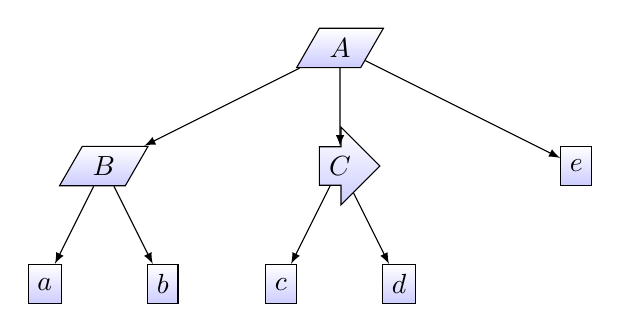
\begin{tikzpicture}[
	level/.style={sibling distance=30mm/#1},
	edge from parent/.style = {draw, -latex},
	sloped,
	every node/.style = {trapezium, trapezium left angle=60, trapezium right angle=-60, draw, align=center, top color=white, bottom color=blue!20,minimum height=0.5cm}
	]
	\node {$A$}  
	child { node {$B$} 
		child{ node [rectangle] {$a$}}
		child{ node [rectangle] {$b$}}
	}    
	child  { node [single arrow] {$C$} 
		child {node [rectangle] {$c$}}
		child {node [rectangle] {$d$}}
	}
	child {node [rectangle] {$e$}}
	;
	
	\end{tikzpicture}
	\caption{Example of a hierarchical plan and its graphical representation.}
	\label{fig:hierarchical plan}
\end{figure}


\begin{example}

Given a task tree $\tau$ as in figure ~\ref{fig:hierarchical plan}, we will compute the duration distribution in the form of PDF for each compound task node including the root node, and then we will return the probability for $\tau$ to satisfy a given deadline $T$. 
First, compute duration distribution for the node $B$. The children task nodes $a,b$, are executed in parallel, therefore we need to find the distribution over the maximum of nodes $a$ and $b$:  
$$P_B(x)=P_{\max(a,b)}(x)=
\begin{cases}
1/16 & x=1 \\
15/16 & x=4 \\
0 & otherwise
\end{cases}$$

Second, compute duration distribution for node $C$. The children task nodes $c,d$, are executed in sequence, therefore, we need to use convolution in order to compute the sum of duration distributions of nodes $c$ and $d$:  
$$P_C(x)=P_{c+d}(x)=
\begin{cases}
1/16 & x=2 \\
3/8 & x=5 \\
9/16 & x=8 \\
0 & otherwise
\end{cases}$$

Last, compute duration distribution for node $A$, the root node. The children task nodes $B,C,e$ are executed in sequence, therefore, we need to use convolution in order to compute the sum of duration distributions of nodes $B$, $C$ and $e$: 
$$P_{\tau}=P_A(x)=P_{A+B+e}(x)=
\begin{cases}
1/1024 & x=4 \\
3/128 & x=7 \\
81/512 & x=10 \\
27/64 & x=13 \\
405/1024 & x=16 \\
0 & otherwise
\end{cases}$$

For every deadline $T$ we can easily return the probability for $\tau$ to satisfy $T$. If $T=8$ the probability is  $F_{\tau}(8)=0.0244$ . 
\end{example}

 
\section{Sum (sequence) nodes}\label{sec:seq}

The size of the support (number of non-zero probability values) of the sum of random variables
may be exponential in the number of variables, even for 2-valued variables.
In fact, as shown in~\cite{}, computing the CDF of a sum of random variables at a given point is NP-hard.
We thus define a notion of approximation, 
which we call an {\bf Kolmogorov upper bound} (defined below),
and supply a $\Trim$ operator that reduces the support size, while 
producing an approximation that is a Kolomogorov upper bound.

Let $X$ and $X'$ be random variables; 
the Kolmogorov distance~\cite{} between $X$ and $X'$ is defined as:
\[
d_K(X,X') = \sup_{x} |F_{X'}(x)-F_X(x)|
\]
Our notion of approximation uses the Kolmogorov distance. Let $1 > \epsilon \geq 0$.
If the following equation holds:
\[
\forall ~ x, ~ F_X(x)+\epsilon \geq F_{X'}(x) \geq F_X(x)
\]
we say that the random variable $X'$ is a Kolmogorov $\epsilon$ upper bound of $X$,
which we denote by $X' \succeq_\epsilon X$. Contrapositively, we call $X$ a  Kolmogorov $\epsilon$ lower
bound of $X$. Note that $X' \succeq_\epsilon X$ implies that $d_K(X,X') \leq \epsilon$,
but not vice-versa.

For example, let $X$ be a r.v. distributed as: $[0.1:1, 0.1:2, 0.8:4]$, and $X'$
a random variable distributed as $[0.2:1, 0.8:4]$. Then we have
$X' \succeq_{0.1} X$. In order to achieve a Kolmogorov upper bound of $\varepsilon $,
the $\Trim$ operator removes  consecutive domain values whose accumulated probability is
less than $\varepsilon$ and adds 
their probability mass to the element in the support that precedes them.

In our  algorithms, the PDF of a r.v. $X$ is represented by a sorted list $D_X$, 
which consists of $d=(x, p')$ pairs, where $x\in \support(X)$
and $p'$ is the probability $P(X{=}x)$. In the pair $d=(x, p')$, we denote the value $x$
by $val(d)$, and the probability $p'$ by $prob(d)$.
If the input $D_X$ to Trim is sorted in increasing order of $x$,
then resulting variable $X'$ (represented by the output $D_{X'}$) 
is a Kolmogorov $\varepsilon$ upper bound of $X$.
(Likewise, if $D_X$ sorted in decreasing order of $x$,
then $X'$ is a Kolmogorov $\varepsilon$ lower bound of $X$.)

%%%%%%%%%%%%%%%%%%%%%
\begin{algorithm}
  \DontPrintSemicolon
  \SetKwFunction{Trim}{Trim}
  \SetKwProg{myproc}{Procedure}{}{}
  \myproc{
  \Trim{$D_X$,$\varepsilon$}
  }{ 
             $D_{X'}=()$, $p=0$ \;	  
  		$d_{prev} = first(D_X)$\;
                $tail = rest(D_X)$ \;
		\While{not-empty($tail$)}{
                        $d = first(tail)$ \;
			\eIf{$p+prob(d) \leq \varepsilon$}{
				$p=p+prob(d)$\;
			}
			{ Append $(val(d_{prev}), prob(d_{prev})+p)$ to $D'$\;
			  $d_{prev} = d$, $p=0$\;
			}
                        $tail=rest(tail)$
                 }
       		 Append $(val(d_{prev}), prob(d_{prev})+p)$ to  $D_{X'}$\;
  \Return $D_{X'}$}
     
\caption{Trim operator}  
\label{alg:Trim}
\end{algorithm}
%%%%%%%%%%%%%%%%%%%%%%%%%%%%%%%%%%%%%%%%%%%%%%%%%%

Trimming decreases the support size, while introducing error. The trick is
to keep the support size under control, while making sure that the error does
not increase beyond a desired tolerance.
Note that the size of the support can also be decreased by simple ``binning'' 
schemes, but these do not provide the desired guarantees.

\noindent We now show that with $D_X$ sorted in increasing order,
$\Trim(X,\varepsilon)$ is an Kolmogorov $\varepsilon$ upper bound of $X$.
\begin{lemma} \label{Trim}
$\Trim(X,\varepsilon)\succeq_\varepsilon X$
\end{lemma}

\begin{proof}
Let $X'=\Trim(X,\varepsilon)$. 
Let $x_1{<}\cdots{<}x_m$ be the support of $X'$. 
Because $\Trim$ adds the probabilities of elements that were removed from the support of $X$ 
to the support element of $X'$ that precedes them, 
we have for all $i$:
\begin{equation}
P_{X'}(x_i) = P_X(x_i) +  P_X(x_i < X < x_{i+1})
\label{collect}
\end{equation}
(assuming $x_{m+1} = \infty$ for convenience.)
The value $P_X(x_i < X < x_{i+1})$ equals the value of $p$ in
the algorithm when the Append is performed, and  the loop invariant $0 \leq p \leq \epsilon$ holds by construction.
For any value $x$, let $l_x=\max\{ i \colon x_i\leq x\}$, thus:
\[
F_{X'}(x) = \sum_{i=0}^{l_x} P_{X'}(x_i)
\]

From Equation~\eqref{collect} we get:
{\small
\begin{align*}
&F_{X'}(x) - F_{X}(x)  \\%[.25cm]
 &{=} \sum_{i=0}^{l-1} (P_{X'}(x_i)- P_X(x_i\leq X <x_{i+1})) \\[-.2cm]
& \hspace{2.7cm}+(P_{X'}(x_{l_x})-P_X(x_{l_x} \leq X \leq x)) \\%[.25cm]
&{=}P_{X'}(x_l) {-} (P(x_l {\leq} X {<} x_{l_x+1}) {-} P(x {<} X {<} x_{l_x+1})) \\
&{=}P(x < X < x_{l_x+1}) \in (0,\varepsilon]
\end{align*}}
\end{proof}



To bound the amount of memory needed for our approximation algorithm,
the next lemma bounds the size of the support of the trimmed r.v.:
%\vspace*{-0.1cm}

\begin{lemma} \label{SizeD}
$|\operatorname{support}(\Trim(X,\varepsilon))| \leq 1/\varepsilon +1$
\end{lemma}

%\vspace*{-0.1cm} 
\begin{proof}
In the Trim operator, each ``Append'' adds 1 to the support of $X'$, and these occur only once inside
the ``else'' statement, and once outside the loop.
The ``else'' part of the loop occurs only if $p+prob(d)> \epsilon$,
after which none of these elements of the list are reused in the ``if'' statement.
Therefore, as the sum of probabilities is 1, then the number of times
the ``else'' part is executed is at most $\frac{1}{\epsilon}$. Thus the total support
is at most $\frac{1}{\epsilon}+1$.
\end{proof}


%Let $X'=\Trim(X,\varepsilon)$ and let $x_1<\cdots<x_m$ be the support of $X'$. 
%And, for notational convenience, let $x_{m+1}=\infty$.
%From the definition of random variable,  $\sum_{x=x_1}^{x_m} P_{X'}(x)=1$. 
%% Gera: removed the above line because it is trivial.
%Let $p_i =\sum_{x_i<x<x_{i+1}} P_X(x)$. Then, $1 = \sum_{i=1}^{m} P_{X'}(x_i) =P_{X}(x_1)+\sum_{i=1}^{m-1} (p_i+ P_{X}(x_{%i+1}))+p_m$.
%According to algorithm~\ref{alg:sequence}, lines 11-12, $p_i \leq \varepsilon $ and $p_i+P_{X}(x_{i+1})>\varepsilon$ for a%ll $0 \leq i < m$. Therefore, $1=\sum_{i=1}^{m} P_{X'}(x_i) > P_{X'}(x_1) + (m-1)\cdot \varepsilon + p_m $. 
%%By direct algebraic manipulation, 
%Using the fact $P_{X'}(x_1)>0$, we get: $(m-1)\cdot \varepsilon<1$, therefore $m\leq 1/\varepsilon$.
%$\Rightarrow m<1/\varepsilon+1 \Rightarrow m\leq 1/\varepsilon$. 

%\vspace*{-0.2cm} 
These lemmas highlight the main idea behind our approximation 
algorithm: the $\Trim$ operator trades off approximation error 
for a reduced size of the support. 

The makespan of a sequence operator is a random variable $X$ the sum 
of the random variables $X_i$ of its children.
Let $Y_i = X_i + Y_{i-1}$ for $1< i \leq n$, and $Y_1=X_1$.
Thus $X$ is distributed as $Y_n$.

As the children of a sequence node may be internal nodes in the task tree,
the input distributions may already be approximations.
Therefore, we compute the random variables $Y'_i = Trim(X'_i + Y'_{i-1}, \varepsilon)$,
where the $X'_i$ is a Kolmogorov $\epsilon_i $ upper bound of $X_i$
and show that $Y'_n$ is a Kolmogorov $\delta $ upper bound of $X$, for an appropriate $\delta $.

The distribution of the sum of random variables $X'_i + Y'_{i-1}$ is 
computed by a discrete convolution, and Trim is computed as in Algorithm~\ref{alg:Trim}.

We begin by bounding the approximation error propagated by convolution (sum of r.v.s):

\begin{lemma} \label{Convolv}
For discrete r.v.s $X_1,X_1',X_2,X_2'$ and $\varepsilon_1,\varepsilon_2 \in [0,1]$, 
if $X_1'\succeq_{\varepsilon_1} X_1$ and  $X_2'\succeq_{\varepsilon_2} X_2$,
then $X_1'+X_2'\succeq_{\varepsilon_1+\varepsilon_2} X_1+X_2$.
\end{lemma}

\begin{proof}
Define error functions $E_1$ and $E_2$ such that 
$F_{X_i'}(x) = F_{X_i}(x)+ E_i(x)$. By construction, we have $ 0 \leq E_i(x) \leq \varepsilon_i$.

By definition of sums of random variables and convolution, we have:
\begin{align*}
& F_{X_1'+X_2'}(y) = \sum_{x=-\infty}^{\infty}F_{X_1'}(y-x)P_{X_2'}(x)\\
&=\sum_{x=-\infty}^{\infty}(F_{X_1}(y-x)+E_1(y-x))P_{X_2'}(x)\\
&= \sum_{x=-\infty}^{\infty}F_{X_1}(y-x)P_{X_2'}(x)+\sum_{x=-\infty}^{\infty}E_1(y-x)P_{X_2'}(x)\\
&\leq\sum_{x=-\infty}^{\infty}F_{X_1}(y-x)P_{X_2'}(x)+\varepsilon_1\sum_{x=-\infty}^{\infty}P_{X_2'}(x)\\
&=\underbrace{\sum_{x=-\infty}^{\infty}F_{X_2'}(y-x)P_{X_1}(x)}_{F_{X_1+X_2'}(x)=F_{X_2'+X_1}(x)}+\varepsilon_1\sum_{x=-\infty}^{\infty}P_{X_2'}(x)\\
&=\sum_{x=-\infty}^{\infty}(F_{X_2}(y-x)+E_2(y-x))P_{X_1}(x) + \varepsilon_1\\
&=\sum_{x=-\infty}^{\infty}F_{X_2}(y-x)P_{X_1}(x)+\sum_{x=-\infty}^{\infty}E_2(y-x)P_{X_1}(x) + \varepsilon_1\\
&\leq\sum_{x=-\infty}^{\infty}F_{X_2}(y-x)P_{X_1}(x)+\varepsilon_2\sum_{x=-\infty}^{\infty}P_{X_1}(x) + \varepsilon_1\\
&\leq F_{X_1+X_2}(y)+\varepsilon_2 + \varepsilon_1\\
\end{align*}

Note that since $E_i(y)$ are non-negative, we also get $F_{X_1'+X_2'}(y) \geq F_{X_1+X_2}(y)$ for all $y$.

\end{proof}

The fact that this trade-off is linear allows us to get a linear approximation error 
in polynomial time, as shown below:


%\vspace*{-0.1cm} 

\begin{theorem}
If $X_i' \succeq_{\varepsilon_i} X_i$ for all $i \in\{1,\dots,n\}$ and $\hat{X}= Sequence(X_1',\dots,X_n', \varepsilon)$ then
$\hat{X} \succeq_e \sum_{i=1}^{n} X_{i}$, where $e={\sum_{i=1}^n\varepsilon_i + n \varepsilon}$. 
\label{appSeqTheorem}
\end{theorem} 
%\begin{theorem}
%If $X_i' \succeq_{\varepsilon_i} X_i$ for all $i \in\{1,\dots,n\}$ and $\hat{X}= Sequence(X_1',\dots,X_n', \varepsilon/n)$ then
%$\hat{X} \succeq_e \sum_{i=1}^{n} X_{i}$, where $e={\sum_{i=1}^n\varepsilon_i + \varepsilon}$. 
%\label{appSeqTheorem}
%\end{theorem} 
%\vspace*{-0.2cm} 

\begin{proof} For $n$ iterations, from Lemma~\ref{Convolv}, we get an accumulated error of 
$\varepsilon_1 +\dots+ \varepsilon_n$. From Lemma~\ref{Trim}, we get an additional error of at most $n\varepsilon$ due to trimming. 
% From Lemma~\ref{SizeD}, $|D|\leq 2n/\varepsilon$ we get overall run-time of $O(\frac{1}{\varepsilon} \cdot n^2 \cdot m)$.
\end{proof}

%\vspace*{-0.3cm} 

\begin{theorem} \label{appSeqComplexTheorem}
Assuming that $m \leq 1/\varepsilon$, the procedure
$Sequence(X_1',\dots,X_n', \varepsilon)$ can be computed
in time $O((nm/\varepsilon)\log(m/\varepsilon))$ using $O(m/\varepsilon)$ memory, where $m$ is the size of the largest support of any of the $X'_i$s.
\end{theorem} 

%\vspace*{-0.3cm} 
\begin{proof}
From Lemma~\ref{SizeD}, the size of list $D$ in Algorithm~\ref{alg:Trim} is at most $m/\varepsilon$
just after the convolution, after which it is trimmed, so the space complexity is $O(m/\varepsilon)$.
$\operatorname{Convolve}$ thus takes time $O((m/\varepsilon)\log(m/\varepsilon))$, where the logarithmic factor
is required internally
for sorting. Since the runtime of  the $\Trim$ operator is linear, and the
outer loop iterates $n$ times, the overall 
run-time of the algorithm is $O((n m/\varepsilon) \log(m/\varepsilon))$.
\end{proof}

%To show that the error bound provided in Theorem~\ref{appSeqTheorem} is tight, we
%demonstrate by the following example 
%that there are $n$ random variables $X_1,\dots,X_n$ for which $Sequence(X_1,\dots,X_n,\varepsilon/n)$ 
%indeed results in error $\varepsilon$.
%\vspace*{-0.2cm} 


%\begin{example}\label{exp:seq}
%The error bound provided in Theorem~\ref{appSeqTheorem} is tight, i.e.
%$Sequence(X_1,\dots,X_n,\varepsilon/n)$ may
%results in error $\varepsilon$:
%Let $0 {\leq} \varepsilon {<}1$ and $n {\in} \mathbb{N}$ such that $1{-}\varepsilon {>} {\varepsilon }/{n}$.
%% i.e.,  $\varepsilon$ is small or $n$ is large. 
%Consider, for very small $\delta>0$, the r.v. $X_1$ defined by:
%$$
%P(X_1{=}x) {=} \begin{cases}
%\delta  & x=0, \\
%{\varepsilon }/{(n (1-\delta )^{x})} & x\in\{1,\dots,n\}, \\
%1{-}\delta{-}\sum_{x=1}^n \frac{\varepsilon }{n(1-\delta )^{x}} & x=n+1, \\
%0 & \text{otherwise}
%\end{cases}
%$$
%and, for $i=2,\dots,n$, let the r.v.s $X_i$ be such that $P(X_i{=}0){=}1{-}\delta$, $P(X_i{=}n^2){=}\delta$, and zero otherwise.
%
%
%\end{example}
%%\vspace*{-.4cm} 

\begin{example}\label{exp:seq}
	Let $0 {\leq} \varepsilon {<}1$ and $n {\in} \mathbb{N}$ such that $1{-}\varepsilon {>} {\varepsilon }/{n}$, i.e.,  
	$\varepsilon$ is small or $n$ is large. 
	Consider, for $\delta>0$ that we will choose to be very small, the random variable $X_1$ defined by
	$$
	P_{X_1}(x) {=} \begin{cases}
	\delta  & x=0, \\
	{\varepsilon }/{(n (1-\delta )^{x})} & x\in\{1,\dots,n\}, \\
	1{-}\delta{-}\sum_{x=1}^n \frac{\varepsilon }{n(1-\delta )^{x}} & x=n+1, \\
	0 & \text{otherwise}
	\end{cases}
	$$
	and, for $i\in\{2,\dots,n\}$, let the random variables $X_i$ be:
	$$
	P_{X_i}(x) =\begin{cases}
	1-\delta  & x=0, \\
	\delta     & x=n^2, \\
	0 & \text{otherwise}
	\end{cases}
	$$
	The distribution of $X=X_1+X_2$ is
	$$
	P_{X}(x) {=} 
	\begin{cases}
	\delta(1-\delta)  & x=0, \\
	{\varepsilon }/{n} & x=1, \\
	{\varepsilon }/{(n (1-\delta )^{x-1})} & x\in\{2,\dots,n\}, \\
	(1{-}\delta)P(X_1{=}n{+}1)& x=n+1, \\
	\delta P(X_1{=}x{-}n^2)& n^2 {\leq} x {\leq} n^2{+}n{+}1 \\
	%\delta P(X_1{=}x{-}n^2)& x{\in}\{n^2, \dots,n^2{+}n{+}1\}, \\
	0 & \text{otherwise}
	\end{cases}
	$$
	The idea here is that the convolution with $X_2$ results in a random variable that is similar in ``shape'' to $X_1$, 
	if we ignore numbers that tend to zero as $\delta$ approaches zero. The convolution also
	modifies the probability $P_{X}1)$ from slightly greater than  $\varepsilon/n$ to precisely $\varepsilon/n$, which will then allow it
	to be trimmed.
	
	Then, if we apply $\Trim(X_1+X_2,\varepsilon/n)$, when $\delta$ is sufficiently small, we get the random variable $X'$ whose probability distribution is:
	$$
	P_{X'}(x) {=} 
	\begin{cases}
	\delta(1-\delta)+{\varepsilon }/{n}  & x=0, \\
	{\varepsilon }/{(n (1-\delta )^{x-1})} & x\in\{2,\dots,n\}, \\
	1-P(X'{<}n+1)& x=n+1, \\
	0 & \text{otherwise.}
	\end{cases}
	$$ 
	
	Note that indeed trimming shifts the mass from $P_X(1)=\varepsilon/n$ to $P_{X'}(0)$.
	This repeats in all steps so, after $n$ steps, we get a random variable $X'$ such that $P_{X'}(0) \xrightarrow{\,\,\delta \to 0\,\,} \varepsilon$. Therefore, 
	$P_{Sequence(X_1,\dots,X_n,\varepsilon/n)}(0) {-} P_{X_1{+}\dots{+}X_n}(0)$
	%\begin{align*}
	%&P(Sequence(X_1,\dots,X_n,\varepsilon/n) {\leq} 0)  \\
	%&             \hspace{4cm} - P(X_1+\dots+X_n \leq 0)
	%\end{align*}
	approaches $\varepsilon$ as $\delta$ approaches zero
	which means that there exists no $\varepsilon' {<} \varepsilon$
	such that $Sequence(X_1,\dots,X_n,\varepsilon/n) \succeq_{\varepsilon'} X_1 + \cdots + X_n$ for all $\delta >0$.
	
\end{example}

A significant advantage of the algorithm we are proposing is that it can be modified to give both an upper and a lower bound for the required probability. In the next paragraph, we describe the way we compute the lower bound and outline the correctness argument. The idea uses the same algorithm suggested (Alg.~\ref{alg:Trim}), but instead of trimming in \textbf{ascending order} (Alg.~\ref{alg:Trim}, line 10) it is performed in \textbf{decreasing order}, starting with the maximum value in the support. The lower bound version of the $\Trim$ operator is referred to as $\LTrim$ (Lower-bound Trim) here, and we provide a proof that $X\succeq_{\varepsilon}\LTrim(X,\varepsilon) $. 
%In this short subsection we will suggest an algorithm which uses the inverted version of $\Trim$ and results a lower bound of the error.
%\begin{center}
%	\begin{algorithm}
%		\DontPrintSemicolon
%		\SetKwFunction{Sequence}{Sequence} 
%		\SetKwFunction{Convolv}{Conv}
%		\SetKwFunction{LTrim}{LTrim}
%		\SetKwFunction{Network}{Network}
%		\SetKwFunction{LNetwork}{LNetwork}
%		\SetKwFunction{Parallel}{Parallel}
%		
%		%\SetKwProg{myalg}{Algorithm}{}{}
%		%-----------------------------------%
%		%\myalg{\Sequence{$D_{Y_1},\dots,D_{Y_n}$ , $T$, $\varepsilon$}}{
%		%$k=n/\varepsilon$\;
%		$D=((0,1))$ //  Dummy random variable: $0$ with probability $1$ \;
%		
%		\For{$i=1$ \emph{\KwTo} $n$} {
%			$D$=Convolve($D, D_{X_i}$)\; 
%			$D$=\LTrim{$D, \varepsilon$}\;
%		}
%		
%		\Return $D$
%		
%		%-------------------------------%
%		\SetKwProg{myproc}{Procedure}{}{}
%		\myproc{
%			\LTrim{$D$,$\varepsilon$}
%		}{ 
%		$D'=()$ \;	  
%		$d_{0} = d_{prev} = \underline{\max \support(D)}$\;
%		$p=0$\;
%		\ForEach{$d \in  \support(D) \setminus \{d_{0}\}$ \underline{in decreasing order}}
%		{			 	
%			\eIf{$p+D[d]\leq \varepsilon$}{
%				$p=p+D[d]$\;
%			}
%			{ Append $(d_{prev}, D[d_{prev}]+p)$ to $D'$\;
%				$d_{prev} = d$\;
%				$p=0$\;}
%		}
%		Append $(d_{prev}, D[d_{prev}]+p)$ to  $D'$\;
%		\Return $D'$}
%	
%	\caption{Sequence ($X_1,\dots,X_n$ , $\varepsilon$)}  
%	\label{alg:sequenceInverse}
%\end{algorithm}
%\end{center}

It is easy to show that a version of $\Sequence$ that keeps the value list of the
random variables sorted in decreasing value 
gives a lower bound on the probability to exceed a deadline. 
Specifically, given a task tree $\tau$, and a random variable $X_\tau$ representing the true 
distribution of the completion time for the network, 
then $X_\tau \succeq_\varepsilon \LNetwork(\tau,\varepsilon)$. The proof is the same as the proof for 
Theorem\ref{alg:approx}, only switch right hand with left hand in each $\succeq_{\varepsilon}$.


\section{Parallel nodes}\label{sec:par}

\SetKwFunction{Parallel}{Parallel}

Unlike sequence composition, the deadline problem for parallel composition
is easy to compute, since the execution time of
a parallel composition is the maximum of the durations:
%\vspace*{-0.2cm}
{\small
\begin{align}
%&P(\max\{X_1,\dots,X_n\}\leq T)= \nonumber \\
F_{\max_{i\in[1:n]}X_i}(T)
%&=P(X_1\leq T \wedge\dots\wedge X_n\leq T)
{=}F_{\bigwedge_{i=1}^n X_i}(T) 
{=}\prod_{i=1}^n F_{X_i} (T)
\label{eq:par}
\end{align}}

\noindent where the last equality follows from independence of the r.v.s.
We denote the construction of the CDF using Equation~\eqref{eq:par} by $\Parallel(X_1,\dots , X_n)$.
If the r.v.s are all discrete with finite support, $\Parallel(X_1,\dots , X_n)$
incurs linear space, and computation time $O(nm log(n))$.

%For the sake of completeness, we will shortly present the $\Parallel(X_1,\dots , X_n)$ algorithm. The notation is the same as in $\Sequence(X_1,\dots , X_n, \varepsilon)$ algorithm.
%
%\begin{algorithm}
%  \DontPrintSemicolon
%  \SetKwFunction{Sequence}{Sequence} 
%  \SetKwFunction{Convolv}{Conv}
%  \SetKwFunction{LTrim}{LTrim}
%  \SetKwFunction{Network}{Network}
%  \SetKwFunction{LNetwork}{LNetwork}
%  \SetKwFunction{Parallel}{Parallel}
%
%   $D=()$\;
%  \ForEach{$x \in  \bigcup_{i=1}^n\support(X_i)$ in ascending order}
%	{$D[x]=\prod_{j=1}^n P(X_j\leq x)$
%	}	
%  
%  \Return $D$
%  
% 
%\caption{Parallel ($X_1,\dots,X_n$)}  
%\label{alg:parallel}
%\end{algorithm}


If the task tree consists only of parallel nodes, one can
compute the exact CDF, with the same overall runtime.
However, when the task tree contain both sequence and parallel nodes we may get
only approximate CDFs as input, and now the above straightforward computation can compound the errors.
When the input CDFs are themselves approximations, we bound the resulting error:

\begin{lemma} \label{appPalTheorem}
For discrete r.v.s $X_1', \dots X_n'$, $X_1, \dots,X_n$, if for all $i=1,\dots,n$,  $X_i' \succeq_{\varepsilon_i} X_i$ and $0\leq\varepsilon_i\leq  \frac{1}{n (K n+1)}$ for some $K>0$,
then, for any $\varepsilon \geq \varepsilon_i$, we have: $\max_{i\in[1:n]}X_i' \succeq_{e} \max_{i\in[1:n]}X_i$ where $e=\sum_{i=1}^n \varepsilon_i + \varepsilon/K$.
\end{lemma}
\begin{proof}
%$P(\max\{X_1',\dots, X_n'\} {\leq} T) {-} P(\max\{X_1,\dots, X_n\} {\leq} T)$
$F_{\max_{i\in[1:n]}X'_i}
 (T) {-} F_{\max_{i\in[1:n]}X_i}
 (T)$
{\small
\begin{align*} 
%&P(\max\{X_1',\dots, X_n'\} {\leq} T) {-} P(\max\{X_1,\dots, X_n\} {\leq} T)\\
%&=\prod_{i=1}^n F_{X_i'}(T)-\prod_{i=1}^n F_{X_i}(T)\\
&\leq \prod_{i=1}^n (F_{X_i}(T)+\varepsilon_i) {-} \prod_{i=1}^n F_{X_i}(T) \\
&\leq \prod_{i=1}^n (1+\varepsilon_i) - 1 
\leq 1+\sum_{i=1}^n \varepsilon_i + \sum_{k=2}^n {n \choose k}  \varepsilon^k - 1 \\
&\leq \sum_{i=1}^n \varepsilon_i + \!\!\!\!\underbrace{\sum_{k=2}^n n^k  \varepsilon^k}_{\text{sum of a geo. series}}\!\!\!\!
\leq \sum_{i=1}^n \varepsilon_i + \frac{n^2 \varepsilon^2}{1-n \varepsilon}
\leq \sum_{i=1}^n \varepsilon_i + \varepsilon/K\\
%\leq (1+\varepsilon)^n  {-} 1 \\
%&= \sum_{k=0}^{n}{n\choose k}\varepsilon ^k - 1  
%\leq \!\!\!\underbrace{\sum_{k=1}^{n} n^k \varepsilon ^k}_{\text{sum of geo. series}} 
%\!\!\!< \dfrac{n\varepsilon}{1-n\varepsilon}
%\leq (1+n)\varepsilon
\end{align*}}
%\vspace*{-0.7cm} 

Since $F_{X_i'}(T) > F_{X_i}(T)$ for each $i$, this expression is nonnegative.
\end{proof}

%Lemma~\ref{appPalTheorem} will allow us to use, for parallel nodes, the efficient computation indicated in Theorem~\ref{TPar}
%provided only that the approximation of the children are good enough, as elaborated in the next section.
%\vspace*{-0.5cm} 

\begin{lemma} \label{tightPalTheorem}
For discrete random variables $X_1', \dots X_n'$, $X_1, \dots,X_n$, if for all $i=1,\dots,n$,  $X_i' \succeq_{\varepsilon_i} X_i$,
then $\max\{X_1',\dots, X_n'\} \succeq_{e} \max\{X_1,\dots,X_n\}$ where $e=1-\prod_{i=1}^n (1-\varepsilon_i)$.
\end{lemma}
\begin{proof}
For any $0<j\leq m$:
{\small
\begin{align*} 
&P(\max\{X_1',\dots, X_n'\} {\leq} T) - P(\max\{X_1,\dots, X_n\} {\leq} T)\\
&=\prod_{i=1}^n F_{X_i'}(T)-\prod_{i=1}^n F_{X_i}(T)\\
&\leq \prod_{i=1}^n F_{X_i'}(T) - \prod_{i=1}^n (F_{X_i'}(T)-\varepsilon_i) \\
&= \prod_{i=1}^n F_{X_i'}(T)- \sum_{S\subseteq \{1,\dots,n\}} \left( \prod_{i\in S}F_{X_i'}(T) \prod_{i\notin S}(-\varepsilon_i) \right)\\
%&=P(X_1' \leq T)\left(\prod_{i=2}^n F_{X_i'}(T)- \sum_{S\subseteq \{1,\dots,n\}, 1\in S} \left( \prod_{i\in S}F_{X_i'}(T) \prod_{i\notin S}(-\varepsilon_i) \right)\right)\\
%&-\sum_{S\subseteq \{1,\dots,n\}, 1\notin S} \left( \prod_{i\in S}F_{X_i'}(T) \prod_{i\notin S}(-\varepsilon_i) \right)\\
&=F_{X_j'}(T)\!\!\underbrace{\left(\!\prod_{\substack{i=1\\i\neq j}}^n \! F_{X_i'}(T)- \!\!\!\!\!\!\!\!\sum_{\substack{S\subseteq \{1,\dots,n\}\\ j\in S}} \!\!\!\! \left( \prod_{i\in S}F_{X_i'}(T) \prod_{i\notin S}(-\varepsilon_i) \right)\!\!\!\right)}_{1}\\
& \hspace{2cm} - \underbrace{\sum_{S\subseteq \{1,\dots,n\}, j\notin S} \left( \prod_{i\in 
S}F_{X_i'}(T) 
\prod_{i\notin S}(-\varepsilon_i) \right)}_{2}
%\\
%&\leq 1-\prod_{i=1}^n (1-\varepsilon_i)
\end{align*}}
We get that, for any $j$, the expression marked as 1 is positive since  we began with a positive 
expression and because the second summand is negative. 
Therefore, taking 1 in place of each $F_{X_j'}(T)$ for every $1 \leq j\leq n$ gives us a larger 
number. This replacement does not affect expression 2 since $F_{X_j'}(T)$ does not participate 
there. 
With this replacement, we get that $F_{X_i'}(T) - F_{X_i}(T)$ is smaller or equal to 
$1-\prod_{i=1}^n 
(1-\varepsilon_i)$ as claimed. Since we also have that $F_{X_i'}(T) - F_{X_i}(T) \geq 
\varepsilon_i \geq 0$ for every $i$, this concludes the proof.
\end{proof}


\begin{example}\label{expl:parallel}
Let $0 {\leq} \varepsilon {<}1$, 
the random variable $X$ defined by
$$
P_{X}(x) =\begin{cases}
1-\varepsilon  & x=0, \\
\varepsilon     & x=1, \\
0 & \text{otherwise}
\end{cases}
$$
The "trimmed" version of $X$ in respect to $\varepsilon$, denoted by $X'$, is:
$$
P_{X'}(x) =\begin{cases}
1  & x=0, \\
0 & \text{otherwise}
\end{cases}
$$
Let $X_1, \dots, X_n$ be $n$ independent copies of $X_1$ and let $X'_1, \dots, X'_n$ be their ``trimmed versions''. Then:
{\small
\begin{align*} 
&F_{\max\{X_1',\dots, X_n'\}}( 0) - F_{\max\{X_1,\dots, X_n\}} (0)\\
&=\prod_{i=1}^n (1)-\prod_{i=1}^n (1-\varepsilon)= 1-\prod_{i=1}^n (1-\varepsilon)
\end{align*}}
If we consider now a task tree with a single parallel aggregation level whose children are $n$ 
sequence nodes where the $i$th sequence node has a single primitive-task child modeled by $X_i$, we get that our
computation will introduce exactly the higher bound predicted by Lemma~\ref{tightPalTheorem}, i.e, this bound is tight.
\end{example}

\section{Task trees: mixed sequence/parallel}

Given a task tree $\tau$ and a accuracy requirement $0<\varepsilon<1$, we generate a distribution for a r.v. $X_{\tau}' $
approximating the true duration distribution  $X_{\tau}$ for the task tree. 
We introduce the algorithm and prove that the algorithm indeed returns an $\varepsilon$-approximation of the completion time of the plan. 
For a node $v$, let $\tau_v $ be the sub tree with $v$ as root and let $child_v$ be the set of children of $v$. 
We use the notation $|\tau|$ to denote the total number of nodes in $\tau$.

\begin{algorithm}
  \DontPrintSemicolon
  \SetKwFunction{Network}{Network} 
  \SetKwFunction{Sequence}{Sequence}
  \SetKwFunction{Parallel}{Parallel}
  
  %-----------------------------------%
  
  {

 Let $v$ be the root of $\tau$  // Hence, $\tau_v=\tau$ \;
	$n_v = |child_v|$ \;
  \If{$v$ is a $\operatorname{Primitive}$ node}{
	\Return the distribution of $v$\;
			}
	
  \If{$v$  is a $\operatorname{Sequence}$ node}{
  	\For{$c \in child_v$} {
	    $X_c$ = \Network($\tau_c$, $\frac{|\tau_c|\varepsilon}{|\tau_v|}$)\;
	 }
	 \Return \Sequence($\{X_c\}_{c \in child_v}$, $\frac{\varepsilon}{n_v|\tau_v|}$)	
	 
	}
			
	\If{$v$ is a $\operatorname{Parallel}$ node}{
	 	\For{$c \in child_v$} {
			$X_c$ = \Network($\tau_c$, $\min(\frac{|\tau_{c}|\varepsilon }{|\tau_v|}   ,\frac{1}{n_v (|\tau_v| n_v+1)})$)\;
		}
		\Return \Parallel($\{X_c\}_{c \in child_v}$)
	}	
  }
%----------------------------------5
  
\caption{Network($\tau$, $\varepsilon$) }\label{alg:approx}
  
\end{algorithm}

%We introduce the algorithm and prove that the algorithm indeed returns an $\varepsilon$-approximation of the completion time of the plan. 
%For a node $v$, let $\tau_v $ be the sub tree with $v$ as root and let $child_v$ be the set of children of $v$. 
%We use the notation $|\tau|$ to denote the total number of nodes in $\tau$.

%Note that given a task tree $\tau$, we can assume, without loss of generality, that there are no parallel nodes as children of parallel nodes, and no sequence nodes as children of sequence nodes, otherwise, we can easily merge them.
Algorithm~2, that implements the operator $\Network$, is a straightforward postorder traversal of the task tree. The only remaining issue is handling the error,  in an amortized approach, as seen in the proof of the following theorem.

\begin{theorem}\label{th:TNapprox}
Given a task tree $\tau$, let $X_{\tau}$ be a r.v. representing the true
distribution of the completion time for the network. Then $\Network (\tau , \varepsilon)\succeq_\varepsilon X_{\tau}$.
\end{theorem}

\begin{proof} 
By induction on $|\tau|$. 
Base: $|\tau|=1$, the node must be primitive, and $\Network$ will just return the distribution unchanged which is obviously an $\varepsilon$-approximation
of itself. Suppose the claim is true for $1 \leq |\tau| < n$. Let $\tau$ be a task tree of size $n$ and
let $v$ be the root of $\tau$. If $v$ is a $\operatorname{Sequence}$ node, by the induction hypothesis that $X_c\succeq_{|\tau_c|\varepsilon/|\tau_v|} X_{\tau_c}$, and by Theorem~\ref{appSeqTheorem}, the maximum accumulated error is 
$\sum_{c \in child_v}
{|\tau_c|\varepsilon}/|\tau_v| + {\varepsilon}/|\tau_v|$ = $(n-1)\varepsilon/|\tau_v|+{\varepsilon}/|\tau_v|= \varepsilon$ for $v$, therefore, $\Sequence(\{X_c\}_{c\in child_v}, {\varepsilon}/{n}) \succeq_\varepsilon X_\tau$ as required. 
If $v$ is a $\operatorname{Parallel}$ node, by the induction hypothesis that $X_c  \succeq_{e_c} X_{\tau_c}$, where $e_c = \min(\frac{|\tau_{c}|\varepsilon}{|\tau_v|}, \frac{1}{n_v (|\tau_v| n_v+1)})$ 
so $\sum_{c\in child_v} e_c \leq   \sum_{c\in child_v} \frac{|\tau_{c}|\varepsilon}{|\tau_v|}  \leq \varepsilon  - \varepsilon/ |\tau_v|  $. Then, by Lemma~\ref{appPalTheorem}, using $K=|\tau_v|$ and $n=n_v$, we get that $\Parallel(\{X_c\}_{c\in child_v})\succeq_\varepsilon  X_\tau$ as required. 
\end{proof}

\begin{theorem}\label{th:TTalgcomplexity}
Let  $N$ be the size of the  task tree  $\tau$,  and $M$ the size of the maximal support of each of the primitive tasks.
If $0 \leq \varepsilon \leq \frac{1}{N (N^2+1)}$ and $M < N/\varepsilon$, the  $\Network$ approximation algorithm 
runs in time $O((N^5 /\varepsilon^2)\log(N^3/\varepsilon^2))$, using
$O(N^3/\varepsilon^2) $ memory.
\end{theorem}

\begin{proof}
The run-time and space bounds can be derived from the bounds on $\Sequence$ and on $\Parallel$, as follows. In the $\Network$ algorithm, the trim accuracy parameter is less than or equal to ${\varepsilon}/{N}$. 
The support size (called $m$ in Theorem~\ref{appSeqComplexTheorem}) of the variables input to $\Sequence$ are $O(N^2/\varepsilon)$.
Therefore, the complexity of the $\Sequence$ algorithm is 
$O((N^4 /\varepsilon^2)\log(N^3/\varepsilon^2))$ and the complexity of the $\Parallel$ operator is $O((N^3/\varepsilon)\log(N))$. The time and space for sequence dominate, so the total time complexity is $N$ times the complexity of $\Sequence$ and the space complexity is that of $\Sequence$.
\end{proof}

If the constraining assumptions on $M$ and $\varepsilon$ in Theorem~\ref{th:TTalgcomplexity} are lifted, the complexity is still polynomial:
replace one instance of $1/\varepsilon$ by $max(m,1/\varepsilon)$, and the other by $max(1/\varepsilon,N (N^2+1))$
in the runtime complexity expression.

\section{Tightening the error estimation}\label{Chap:Bound}

Until now, we presented an approximation algorithm (\Network) and provided a bounds for time-accuracy trade-offs. In some cases, however, our algorithm provides results that are much more accurate than promised. This may be wasteful, because this extra precision comes with a price on runtime.

In this section we propose a tighter analysis. The term tight here means 
that we provide the smallest error estimation based only the structure of the tree. 
In other words, given a task tree we provide the smallest error bound that is true for any choice 
of the leaves, i.e., the random variables.


Consider, as an extreme example, a simple task tree with a sequence node at the root and below it only parallel nodes. The total error of our approximation algorithm (\Network) in this case is only due to the invocation of \Sequence at the tail of the recursion. The \Network algorithm acts as if all the other nodes add additional errors. Eventually, the \Sequence
computation produces a very small error which takes the toll of an excessive computation time. 

%We will present now a recursive approximation algorithm with a tighter bound on the error parameter 
%for every sequence node, called $\NetworkTight(\tau, 
%\varepsilon_0)$. The parameters to this algorithm are %as for \Network, i.e., 
%a task tree $\tau$ and 
%$\varepsilon_0$ which is the upper bound on the error produced by the tree. The approach here is to 
%define the system of equations $ \tau_v(\overrightarrow{\varepsilon}) $ which forms the polynomial 
%$p_v$ (Lemma~\ref{lemma:poly}) where $v$ is a node in $\tau$, and the variables are the error 
%bounds we require for each invocation of the \Sequence method represented by the vector 
%$\overrightarrow{\varepsilon}$. We then propose to solve the inequality $p_v \leq \varepsilon_0$ and calculate the 
%root node distribution using the solution. The method used for solving these inequality, with an exact or numeric tool, is orthogonal to the analysis in this paper. 
%We will prove that the proposed algorithm provides a tight bound for some task trees, assuming that 
%the solution is exact. 
%For a task tree $\tau $ that contains $n_s$ sequence nodes, we define a recursive system of equations, $ \tau_v(\overrightarrow{\varepsilon}) $ and by that the polynomial $p_v$, with the variables $\overrightarrow{\varepsilon} =\varepsilon_1 \dots \varepsilon_{n_s}$ where each $\varepsilon_i\in [0,1],  1\leq i \leq n_s $ is associated with the corresponding $i$'th sequence node $v_i$.
%Given a task tree $\tau$ and $\varepsilon_0$, \NetworkTight($\tau$, $\varepsilon_0$) made of three methods. First, construct the polynomial $ p_v $ by using the method \EstimateError($\tau$), second, find $p_v \leq \varepsilon_0$ roots by solving this inequality with any solving tool (numeric solver, exact solver, etc.). Finally, use the root values $\varepsilon_1 \dots \varepsilon_{n_s}$ calculated by the solver to compute the approximated distribution derived from $\tau$ by using the method \CalcNetwork($\tau$, $\varepsilon_1, \dots, \varepsilon_{n_s}$).
%The construction of the polynomial $p_v$ is outlined in \EstimateError($\tau$), Algorithm~\ref{alg:BuildPolynomial}. The solver method is open for the user: he or she can use any algorithm for the purpose, any solution will do. 
%The \CalcNetwork($\tau$, $\varepsilon_1, \dots, \varepsilon_{n_s}$) method is a second pass over the tree. It uses the solution of the 
%polynomial roots to calculate the approximated distribution. Actually, 

We will present now a recursive approximation algorithm with a tighter bound on the error parameter for every sequence node. 
First, we present the algorithm $\EstimateError$ that computes the approximation error for a tree $\tau$ given a function $\varepsilon$ that maps each of the network nodes in $\tau$ to the parameter passed in line 7 of the $\Network$ procedure, i.e., we use a generalized version of $\Network$, called $Network2$. 

The main property of this algorithm is as follows:

\begin{theorem}\label{theorem:approxEps0}
	For a task tree $\tau$ and $\varepsilon_1, \dots, \varepsilon_{n_s}$, let 
	$\varepsilon_0=p_v(\varepsilon_1, \dots, \varepsilon_{n_s}) $ where $p_v=\EstimateError(\tau)$, 
	and let $X_{\tau}$ be a random variable representing the true
	distribution of the completion time for $\tau$. Then,
	$\CalcNetwork(\tau, \varepsilon_1, \dots, \varepsilon_{n_s}) \succeq_{\varepsilon_0} X_{\tau}$.
\end{theorem}

\begin{proof}
	By induction over the depth of $\tau$ denoted by $d$. Base: $ d=1$, a single primitive node $ v_p 
	$. Primitive nodes do not carry any error, and by procedure \EstimateError line 3, $P_{v_p}=0$, 
	therefore  $\CalcNetwork(\tau_{v_p}) \succeq_0 X_{\tau_{v_p}}$. 
	Induction hypothesis: Assume the lemma is true for a task tree with depth $ <d $. Step: we refer to the children nodes of the root node $\ch(v_{root})= \lbrace c_1, c_2,...,c_{|\ch(v_{root})|}\rbrace$ as a set of sub task trees, each of them with depth smaller than $ d $ and $\varepsilon_{c_1}=(\varepsilon_{c_1,1}, \dots,\varepsilon_{c_1,n_s})$ $, \dots, $  $\varepsilon_{c_{|\ch(v_{root})|}} = (\varepsilon_{c_{|\ch(v_{root})|},1}, \dots, \varepsilon_{c_{|\ch(v_{root})|},n_s})$ accordingly. 
	%$\overrightarrow{\varepsilon}_{c_1}, \dots, \overrightarrow{\varepsilon}_{c_{|\ch(v_{root})|}} $
	If $v_{root}$ is a sequence node then,
	by Theorem~\ref{appSeqTheorem}, sequence node produce an error which is the sum of all children nodes error and an additional $\varepsilon_{v_{root}}$ caused by the trim operator $P_{v_{root}}={\sum_{c \in \ch(v_{root})}{P_{c}}+ \varepsilon_{v_{root}}}$ equivalent to \EstimateError line 7. By the induction hypothesis, each of the children sub trees satisfy the lemma and we get that:$ \CalcNetwork(\tau_{v_{root}}, \varepsilon_{c_1}, \dots, \varepsilon_{c_{|\ch(v_{root})|}})$ $\succeq_{P_{v_{root}}(\varepsilon_{c_1}, \dots, \varepsilon_{c_{|\ch(v_{root})|}})} X_{\tau_{v_{root}}} $ as required.
	
	If $v_{root}$ is a parallel node then,
	by Lemma~\ref{tightPalTheorem}, $P_{v_{root}}=1-\prod_{c \in \ch(v_{root})}{(1-P_{c})}$ equivalent to \EstimateError line 11. By the induction hypothesis, each of the children sub trees satisfy the lemma and we get that:$ \CalcNetwork(\tau_{v_{root}}, \varepsilon_{c_1}, \dots, \varepsilon_{c_{|\ch(v_{root})|}})$ $\succeq_{P_{v_{root}}(\varepsilon_{c_1}, \dots, \varepsilon_{c_{|\ch(v_{root})|}})} X_{\tau_{v_{root}}} $ as required.
\end{proof}

%Our approach here is to assign a variable $\varepsilon_i$ to each node, representing the maximal error that this node may produce. Then, we propose to compute an inequality that these errors must satisfy if we want the total error of the tree to be below some given $\varepsilon_0$. This inequality is of the form $p_{v} \leq \varepsilon_0$ where $p_v$ is a polynomial that is defined recursively for each node, eventually also for the root node. 

------------------------





is to compute an inequality over the a set of variables


a system of equations  which forms the polynomial $p_v$ (Lemma~\ref{lemma:poly}) where $v$ is a node in $\tau$, and the variables are the error 

bounds we require for each invocation of the \Sequence method represented by the vector 
$\overrightarrow{\varepsilon}$. The next step is to solve the inequality $p_v \leq \varepsilon_0$ and calculate the 
root node distribution using the solution. The method used for solving these inequality, with an exact or numeric tool, is orthogonal to the analysis in this paper. 
We will prove that the proposed algorithm provides a tight bound for some task trees, assuming that 
the solution is exact. 
For a task tree $\tau $ that contains $n_s$ sequence nodes, we define a recursive system of equations, $ \tau_v(\overrightarrow{\varepsilon}) $ and by that the polynomial $p_v$, with the variables $\overrightarrow{\varepsilon} =\varepsilon_1 \dots \varepsilon_{n_s}$ where each $\varepsilon_i\in [0,1],  1\leq i \leq n_s $ is associated with the corresponding $i$'th sequence node $v_i$.
Given a task tree $\tau$ and $\varepsilon_0$, the algorithm \NetworkTight($\tau$, $\varepsilon_0$) calls sequentially to three methods. First, build the polynomial $ p_v $ by using the method \EstimateError($\tau$). Second, find $p_v \leq \varepsilon_0$ roots by solving this inequality with any solving tool (numeric solver, exact solver, etc.). Finally, use the root values $\varepsilon_1 \dots \varepsilon_{n_s}$ calculated by the solver to compute the approximated distribution derived from $\tau$ by using the method \CalcNetwork($\tau$, $\varepsilon_1, \dots, \varepsilon_{n_s}$).
The construction of the polynomial $p_v$ is outlined in \EstimateError($\tau$), Algorithm~\ref{alg:BuildPolynomial}. The solver method is open for the user: he or she can use any algorithm for the purpose, any solution will do. 
The \CalcNetwork($\tau$, $\varepsilon_1, \dots, \varepsilon_{n_s}$) method is a second pass over the tree. It uses the solution of the 
polynomial roots to calculate the approximated distribution. Actually, \CalcNetwork($\tau$, $\varepsilon_1, \dots, \varepsilon_{n_s}$) algorithm is very similar to \Network($\tau$, $\varepsilon_0$) algorithm, except two significant differences. The first, syntactic,  \CalcNetwork parameters are the tree $\tau$ and the errors (root values of $p_v \leq \varepsilon_0$) computed by the solver, therefore, in every recursive call a subtree $\tau_c$ is sent but the list of errors is re-sent with every invocation. The second, is the essence of this algorithm, when the \Sequence method is called for node $v$, we already know the error caused by this exact sequence node operator therefore we pass the $\varepsilon_v $ error from the list $\varepsilon_1, \dots, \varepsilon_{n_s}$.
\EstimateError($\tau$) run-time complexity is $n$, one pass on every node in the tree $\tau$.  \CalcNetwork($\tau$, $\varepsilon_1, \dots, \varepsilon_{n_s}$) run-time complexity is the same as for \Network($\tau$).
\begin{algorithm}
  \DontPrintSemicolon
  \SetKwFunction{Sequence}{Sequence}
  \SetKwFunction{Parallel}{Parallel}
  \SetKwFunction{BuildPolynomial}{BuildPolynomial}
  %-----------------------------------%
  {

 Let $v$ be the root of $\tau$\;
  \If{$v$ is a $\operatorname{Primitive}$ node}{
	\Return $0$ \;
			}
	
  \If{$v$  is a $\operatorname{Sequence}$ node}{
  	\For{$c \in child(v)$} {
	    $e_c=$ \EstimateError($c$, $\varepsilon$)\;
	 }
	 \Return $\varepsilon(v) + \sum_{c\in child(v)}e_{c}$	
	}
	\If{$v$ is a $\operatorname{Parallel}$ node}{
	 	\For{$c \in child(v)$} {
	    $e_c=$ \EstimateError($c$, $\varepsilon$)\;
	 }
		\Return $1-\prod_{c\in child(v)} (1-e_{c})$
	}	
  }
%----------------------------------5
  
\caption{EstimateError($\tau$, $\varepsilon$) }
\label{alg:BuildPolynomial}
  
\end{algorithm}


\begin{algorithm}
  \DontPrintSemicolon
  \SetKwFunction{Network}{Network} 
  \SetKwFunction{Sequence}{Sequence}
  \SetKwFunction{Parallel}{Parallel}
  
  %-----------------------------------%
  
  {

 Let $v$ be the root of $\tau$\;
  \If{$v$ is a $\operatorname{Primitive}$ node}{
	\Return the distribution of $v$\;
			}
	
  \If{$v$  is a $\operatorname{Sequence}$ node}{
  	\For{$c \in child(v)$} {
	    $X_c$ = \CalcNetwork($\tau_c$, $\varepsilon$)\;
	 }
	 \Return \Sequence($\{X_c\}_{c \in child(v)}$, $\varepsilon(v)$)	
	 
	}
			
	\If{$v$ is a $\operatorname{Parallel}$ node}{
	 	\For{$c \in child(v)$} {
			$X_c$ = \CalcNetwork($\tau_c$, $\varepsilon$)\;
		}
		\Return \Parallel($\{X_c\}_{c \in child(v)}$)
	}	
  }
%----------------------------------5
  
\caption{Network2($\tau$, $\varepsilon$) }
\label{alg:calc}
  
\end{algorithm}

\begin{lemma}\label{lemma:poly}
Given a task tree $\tau$, the system of equations $ \tau_v(\overrightarrow{\varepsilon}) $ is a polynomial of $\overrightarrow{\varepsilon}$, with maximal degree ${n_s}$, the number of sequence nodes in $\tau$.  
\end{lemma}
\begin{proof}
We will prove by induction over the depth of $\tau$ denoted by $d$. Base: $ d=1$, a single primitive node $ v_p $. $\tau_{v_p}(\varepsilon)=0$, polynomial with degree 0.
Induction hypothesis: Assume the system of equations of a task tree with depth $ <d $ is polynomial, with maximal degree as the number of sequence nodes in the task tree. Step: we refer to the children nodes of the root node $\ch(v_{root})= \lbrace c_1, c_2,...,c_{|\ch(v_{root})|}\rbrace$ as a set of sub task trees, each of them with depth smaller than $ d $. If $v_{root}$, is a sequence node then $\tau_{v_{root}}(\varepsilon)=\sum_{i=1}^{|\ch(v_{root})|}\tau_{c_i}(\varepsilon) +  \varepsilon$, thus by the inductive hypothesis the system of equations, $ \tau_{c_i} $, each a sub-tree with root $ c_i $ is polynomial with a maximal degree of the number of sequence nodes. Therefore, $\tau_{v_{root}}(\varepsilon)$ is also polynomial since polynomial is closed under addition, farther more, the polynomial degree is the maximum degree between $\left( \tau_{c_1}(\varepsilon) \dots \tau_{c_{|\ch(v_{root})|}}(\varepsilon)\right)$, which is smaller than the number of sequence nodes in the task-tree. If $v_{root}$, is a parallel node then $\tau_{v_{root}}(\varepsilon)=1-\prod_{i=1}^{|\ch(v_{root})|} (1-\tau_{c_i}(\varepsilon))$ , thus by the inductive hypothesis the system of equations, $ \tau_{c_i} $, each sub-tree with root $ c_i $ is polynomial with a maximal degree of the number of sequence nodes. Therefore, $\tau_{v_{root}}(\varepsilon)$ is also polynomial since polynomial is closed under multiplications, farther more, the degree is the sum of all polynomial degrees, $\left( \tau_{c_1}(\varepsilon) \dots \tau_{c_{|\ch(v_{root})|}}(\varepsilon)\right)$, which is in the worst case, the number of sequence nodes under the $v_{root}$. 
\end{proof}


%The following Lemmas, shows that by solving the system of equation $\tau_v(\varepsilon)$ with the variables $\varepsilon_1 \dots \varepsilon_m$ and assuming that $\varepsilon_1=\varepsilon_2= \dots =\varepsilon_m$ we can uniquely determine the error needed to be given for each sequence node in task tree $\tau$. Assuming that $\varepsilon_1=\varepsilon_2= \dots =\varepsilon_m$ do not promise a tight bound but a unique solution, in order to get the tight bound we have to take into consideration the tree structure, this can be handled as future work.

%\begin{lemma}\label{lemma:sysEq}
%
%
%The system of equations $\tau_v(\varepsilon)$ solution gives a tight bound on the error.
%\end{lemma}
%\begin{proof}
%Primitive nodes do not carry any error, therefore, in procedure \EstimateError , line 3, we can see the error is 0. By Theorem~\ref{appSeqTheorem}, sequence node produce an error which is the sum of all children nodes error and an additional $n\varepsilon$ caused by the trim operator, equivalent to \EstimateError, line 7. By Lemma~\ref{palTheorem}, parallel node slightly increases the error as a function of the children nodes error equivalent to \EstimateError, line 11.
%\end{proof}


\begin{theorem}\label{theorem:tight}
There is a task tree $\tau$, a bound $T$, and numbers $\varepsilon_1, \dots, \varepsilon_{n_s}$ 
such that $F_{\CalcNetwork(\tau, \varepsilon_1, \dots, \varepsilon_{n_s})}( T) - F_{X_\tau}(T) = \varepsilon_0$ where $\varepsilon_0=p_v(\varepsilon_1, \dots, \varepsilon_{n_s}) $,
$p_v=\EstimateError(\tau)$, and $X_\tau$ is the distribution of the completion time of $\tau$. 
\end{theorem}
\begin{proof}
See Example~\ref{exp:seq} and Example~\ref{expl:parallel}.
\end{proof}

% Gera: add discussion here


The above result establishes that $\CalcNetwork$ is tight in the sense that there is no $\varepsilon < \varepsilon_0$ 
such that $\CalcNetwork(\tau, \varepsilon_1, \dots, \varepsilon_{n_s})$ is always $\succeq{\varepsilon_0}$ than $X_{\tau}$. 
If we look more closely at on the examples used
to prove the theorem, we can say more about the tightness of our algorithm, as follows.
Since the examples consist of task trees whose root nodes are both of
type sequence and of type parallel, we get that any algorithm that traverses the tree
recursively like we do, cannot do better than $\CalcNetwork$ in terms of computing a
random variable that is $\succeq{\varepsilon}$ than $X_{\tau}$ with a smaller $\varepsilon$. 
More formally, if we restrict the discussions to algorithms where the trimming of the variables in a subtree
depend only on the structure of the subtree (not on siblings or parents or the CDFs of the variables), then 
$\CalcNetwork$ applies the maximal possible trimming (assuming that we have an optimal solution to $\EstimateError$). 
This means that $\CalcNetwork$ is an improvement over 
$\Network$ (Algorithm~\label{alg:approx}) that satisfies this assumption. 
Practically, the improvement is in allowing more trimming and, by that, saving unnecessary computations. 
Specifically, both $\CalcNetwork$ and $\Network$ are guaranteed to give a satisfactory answer but they may sometimes compute 
an approximation that is better than required in the price of taking more run-time. $\CalcNetwork$ is better in that it
takes this extra time only in cases where any algorithm that decides how to trim based only on the shape of the subtree 
(and not on the CDFs of the random variables or on other parts of the tree) would.
%The above result establishes that $\CalcNetwork$ is tight in the sense that there is no $\varepsilon < \varepsilon_0$ such that $\CalcNetwork(\tau, \varepsilon_1, \dots, \varepsilon_{n_s})$ is always $\succeq{\varepsilon_0}$ than $X_{\tau}$. It does not say (because it is not true) that this is always
%the case, only that there are task trees for which there is no $\varepsilon < \varepsilon_0$ for which the $\succeq{\varepsilon_0}$ relation is satisfied.
%
%If we look more closely at Theorem~\ref{theorem:tight} and on the examples used
%to prove the theorem, we can say more about the tightness of our algorithm.
%Since the counter examples consist of task trees whose root nodes are both of
%type sequence and of type parallel, we get that any algorithm that traverses the tree
%recursively like we do, cannot do better than $\CalcNetwork$ in terms of computing a
%random variable that is $\succeq{\varepsilon}$ than $X_{\tau}$ with a smaller $\varepsilon$. 
%This is because any algorithm that handles a subtree without its context must... 
%
%
%
%
%Our goal was to suggest a tighter bound approximation algorithm and we chose to calculate the bound 
%separately for sequence nodes and parallel nodes. By separating those cases and separately 
%calculating the bound on the error, we could suggest a recursive algorithm $\NetworkTight(\tau, 
%\varepsilon_0)$ such that given a task tree $\tau$ and a upper bound $\varepsilon_0$, 
%$\NetworkTight (\tau , \varepsilon_0)\succeq_{\varepsilon_0} X_{\tau}$. Clearly, from 
%theorem~\ref{theorem:approxEps0} we know that $ \CalcNetwork(\tau, \varepsilon_1, \dots, 
%\varepsilon_{n_s}) \succeq_{p_v(\varepsilon_1, \dots, \varepsilon_{n_s})} X_{\tau} $, and by using 
%any kind of \Solve method we know that $p_v(\varepsilon_1, \dots, \varepsilon_{n_s})\leq 
%\varepsilon_0$, then we get that $\NetworkTight (\tau , \varepsilon_0)\succeq_{\varepsilon_0} 
%X_{\tau}$. In addition to the correctness of the algorithm, we also established that there are 
%cases where the bound is tight, such as in theorem~\ref{theorem:tight}, the tightens shown by two 
%concrete examples. Moreover, we argue that given the constraint of separately calculating the bound 
%on the error for sequence nodes and parallel nodes, this algorithm, $\NetworkTight(\tau, 
%\varepsilon_0)$, is as tight as it gets, otherwise, the examples would not be applicable. As future 
%work we strongly suggest to consider the option of calculating the distribution not by differing 
%sequence nodes from parallel nodes but treat the task tree in more of a holistic manner. 



\section{Complexity results}\label{sec:complexity}

We show that the deadline problem is NP-hard, 
even for a task tree consisting only of primitive tasks and one sequence node, i.e.
{\em linear plans}~\cite{Russell:2003:AIM:773294,simmons2001planning,aktolga2004java}. 
%We begin with a lemma on sums of random variables.

  %(we call the following problem SumDiscreteRV).
\begin{lemma} \label{SumDiscreteRV}
Let $Y=\{Y_1,\dots,Y_n\}$ be a set of discrete real-valued r.v.s specified by probability mass functions 
with finite supports, $T \in \mathbb{Z}$, and $p\in[0,1]$. Then, deciding  whether $F_{\sum_{i=0}^{n} Y_{i}}(T)>p $ is NP-Hard.
\end{lemma}

\begin{proof} 
First proved in~\cite{mohring2001scheduling} by a reduction from \textit{Partition}~\cite[problem number SP]{Garey:1990:CIG:574848} and also shown in~\cite{cohen2015estimating}, by reduction from \textit{SubsetSum}~\cite[problem number SP13]{Garey:1990:CIG:574848}.
%Recall that
%$\textit{SubsetSum}$ is: given a set $S=\{s_{1},\dots,s_{n}\}$ of integers, and integer target value $T$, is there a subset of $S$ whose sum is exactly $T$? 
%Given an instance of \textit{SubsetSum}, create
%the two-valued r.v.s $Y_{1},\dots,Y_{n} $ with $P(Y_i=s_i)=1/2$ and $P(Y_i=0)=1/2$. 
%By construction, there exists a subset of $S$ summing to $T$ if and only if $P(\sum_{i=0}^{n} Y_{i}=T)>0$.
%
%Suppose that algorithm $ A(Y,T,p) $ can decide $P(\sum_{i=0}^{n} Y_{i}<T)>p $ 
%in polynomial time. Then, since the r.v.s $Y_i$ are two-valued uniform r.v.s, the only possible values of $p$ are integer multiples of ${1}/{2^n}$,
%and we can compute $p=P(\sum_{i=0}^{n} Y_{i}<T)$ using a binary search on $p$ using $n$ calls to $A$.
%To determine whether $P(\sum_{i=0}^{n} Y_{i}=T)>0$, simply use this scheme twice, since $P(\sum_{i=0}^{n} Y_{i}=T)>0$
%is true if and only if $P(\sum_{i=0}^{n} Y_{i}<T) < P(\sum_{i=0}^{n} Y_{i}<T+1)$.
\end{proof}
 
\begin{theorem}
Deciding if the probability that a task tree satisfies a deadline $T$ is above a threshold $p$ is NP-hard.
\end{theorem}

\begin{proof} The makespan of task tree consisting of a single sequence node with $n$ leaf nodes is the sum of $n$ random variables (the completion times of the leaves). Therefore, the theorem follows immediately from Lemma~\ref{SumDiscreteRV}. 
\end{proof}

Our next goal is to show that not only that the above decision problem is NP-hard but also to analyze the hardness of computing the exact probability $F_{\sum_{i=0}^{n} Y_{i}}(T)$. To this end, we note that 
if $Pr(Y_i=y)=1/|\support(Y_i)|$ for every $i$ and every $y\in\support(Y_i)$, computing the probability $F_{\sum_{i=0}^{n} Y_{i}}(T)$ is equivalent, up to scaling by $\prod_{i=1}^n |\support(Y_i)|$, to counting the number of assignments to the random variables  such that $\sum_{i=0}^{n} Y_{i} \leq T$. 

\begin{definition} 
	Given the random variable $Y_1,\dots,Y_n$ and a deadline $T$,
	the \#deadline-probability counting problem is to count the number of assignments to the random variables such that $\sum_{i=0}^{n} Y_{i} \leq T$.
\end{definition}

It is easy to see that \#deadline-probability is in \#P because we can check if an assignment satisfies $\sum_{i=0}^{n} Y_{i} \leq T$ in linear time.

We will show that \#deadline-probability is \#P-complete by providing a reduction from \#knapsack. Recall the definition of $\#\operatorname{knapsack}$~\cite{arora2009computational}: We are given $n$ objects, and together with each object $i\in \{1,\dots , n\}$ we have its integer weight $w_i$, and the total weight $W$ our knapsack can hold. Our objective is to find the number of subsets $K \subseteq \{1, \dots , n\}$ such that $\sum_{i \in K} w_i \leq W$. We call the sets satisfying this weight constraint feasible, and denote them as $S$. Thus, the \#knapsack problem is to compute $|S|$.

\begin{theorem} \label{deadlinSP}
\#deadline-probability is \#P-complete.
\end{theorem}

\begin{proof} By reduction from \#knapsack. Given an instance of \#knapsack, create the two-valued random variables $Y_{1},\dots,Y_{n} $ with $P(Y_i=w_i)=1/2$ and $P(Y_i=0)=1/2$ and choose $T=W$. By construction, $|S|=2^n \cdot F_{\sum_{i=1}^{n} Y_{i}}(T)$ (where $S$ is as explained above). Since, every assignment is chosen with probability $1/2^n$, we get that $|S|$ is the number of assignments such that $\sum_{i=1}^{n} Y_{i} \leq T$. Thus, if we could count the number of such assignments, we could also count the size of $S$. This establishes that the problem is \#P-complete. 
\end{proof}

Finally, we consider the linear utility function, i.e. the problem
of computing an expected makespan of a task network.
Note that although for linear plans the {\em deadline problem} is NP-hard, the {\em expectation problem} is trivial because the expectation
of the sum of r.v.s $X_i$ is equal to the sum of the expectations of the $X_i$s.
For {\em parallel nodes}, it is easy to compute the CDF and therefore also easy to
compute the expected value.
Despite that, for task networks consisting of {\em  both} sequence nodes and
parallel nodes, these methods cannot be effectively combined, and in fact, we have:
\begin{theorem}
Computing the expected completion time of a task network is NP-hard.
\end{theorem}

\begin{proof}
By reduction from subset sum. Construct r.v.s (``primitive tasks'') $Y_i$ as in the proof of Lemma~\ref{SumDiscreteRV}, and denote
by $X$ the r.v. $\sum_{i=1}^{n} Y_{i}$. Construct one parallel node
with two children, one being the a sequence node having the
completion time distribution
defined by $X$, the other being a primitive task that has a completion time
$T_j$ with probability 1. (We will use more than one such case,
which differ only in the value of $T_j$, hence the subscript $j$).
Denote by $M_j$ the r.v. that represents the completion time
distribution of the parallel node, using this
construction, with the respective $T_j$. Now consider computing the
expectation of the $M_j$ for the following cases: $T_1 = T+{1}/{2}$
and $T_2 = T+{1}/{4}$.
Thus we have, for $j\in\{ 1, 2\}$, by construction and the definition of
expectation:
{\small
\begin{eqnarray*}
E[M_i] &=& T_j F_{X}( T_j) + \sum_{x > T_j} x~P_{X}(x)  \\
          &=& T_j F_{X}( T)+ \sum_{x \geq T+1} x~P_{X}(x)
\end{eqnarray*}}
where the second equality follows from the $Y_i$ all being
integer-valued r.v.s (and therefore $X$ is also integer valued).
Subtracting these expectations, we have $E[M_1]-E[M_2]=\frac{1}{4}F_{X}( T)$.
%\begin{eqnarray*}
%(T+\frac{1}{2}) F_{X}( T) + \sum_{x \geq T+1} x P(X=x) - \\
%(T+\frac{1}{4}) F_{X}( T) + \sum_{x \geq T+1} x P(X=x) 
%\end{eqnarray*}
%which reduces to $\frac{1}{4}F_{X}( T)$. Therefore, using the computed expected values, we can compute
Therefore, using the computed expected values, we can compute
$F_{X}( T)$, and thus also $P(X=T)$, in polynomial time.
%Using two such computations,  we can also compute $P(X=T)$,
%and the latter is non-zero if and only if there is a subset of $S$
%summing to $T$.
\end{proof}

Parallel composition does not bear the complexity that we found in sequential composition. Namely, we show that if all the compound tasks in the plan are $\parl$, we can decide the duration problem efficiently. The center column in the table.

\begin{lemma} \label{TPar}
	Let $Y=\{Y_1,\dots,Y_n\}$ be a set of independent random variables specified by the same type of %probability distribution functions 
	CDF (either all are Discrete, all are Normal, or all are Piecewise polynomial) and let $T \in \mathbb{R}$. Then, deciding $P(\max\{Y_1,\dots,Y_n\} \leq T) $ 
	%and $P(\min\{Y_1,\dots,Y_n\}\leq T) $ 
	can be done in polynomial-time.\footnote{Here, we measure the size of the input by $n$, the number of random variables, and by the variable $m$, the (maximal) size of the support of each of the variables. The run time is polynomial in both variables.}
\end{lemma}

\begin{proof}
	The CDF of $Y_{max} =\max\{Y_1,\dots,Y_n\} $, by definition, 
	\begin{align*}
	F_{Y_{max}}(T)= &P(Y_{max}\leq T)\\
	= & F_{\max\{Y_1,\dots,Y_n\}}(T)\\
	= & P(\underbrace{Y_1<T \wedge\dots\wedge Y_n\leq T}_\text{i.d.})\\
	= & F_{Y_1}(T)\cdots F_{Y_n}(T)
	\end{align*} 
	
	
	In conclusion, we get that $F_{Y_{max}}(T) = F_{Y_1}(T)\cdots F_{Y_n}(T)$ which gives us a linear-time algorithm for computing the maximum.
\end{proof}

We summarized our results by analyzing how the different plan structures together with different execution time distribution effects on the computational complexity. Specifically, complexity of the deadline problem depends on:

\begin{itemize}
	\item \textbf{The structure of the plan}: Whether the tasks are executed in a sequence, in parallel or in a combination of sequential and parallel execution (which we  call ``mixed");
	\item \textbf{Tasks execution time distribution }:  Whether we deal with discrete probability distribution, piecewise polynomial distribution(of which uniform distribution is a special case) or normal distributions.  
\end{itemize}
The following table shows the complexity of answering the deadline problem for all possible combinations of structure vs. distribution:
\begin{table}[h]
	\begin{center}
		\begin{tabular}{  p{1.6cm} || p{1.5cm} |p{2cm} | p{1.6cm} |}
			%    \hline
			\diag{.1em}{1.6cm}{Dist} {Struct}  &  Sequential & Parallel & Mixed \\ \hline \hline
			Discrete & NP-hard (Lemma~\ref{SumDiscreteRV})&  Polynomial (Lemma ~\ref{TPar}) & NP-hard (Lemma~\ref{SumDiscreteRV}) \\ \hline
			{Piecewise Polynomial} & NP-hard  & Polynomial (Lemma ~\ref{TPar}) &  NP-hard \\ \hline
			Normal &  Polynomial (Sum of Normal random variables) & Polynomial  &  We don't know :-(\\
			\hline
			
		\end{tabular}
		
	\end{center}
	\caption{Plan Structure vs. Distribution}
	\label{Tab:comp}
\end{table}

Essentially the table shows that the main complexity in our domain is combinatorial, i.e., that an algorithm for answering the duration problem, in most cases, cannot do better than enumerating all combinations of task durations. Note, we could not determine the complexity of a mixed plan when all task nodes are normally distributed. 


\section{Empirical Evaluation}\label{sec:exp}


%\begin{table}[tbh]
%{\tiny
%\begin{tabular}{|l|l|l|| p{1.5cm}|p{1.5cm}|p{2.4cm}||l|l|l|l|l|}
%\hline
%\multicolumn{1}{|c|}{\multirow{2}{*}{Task Tree}} & \multicolumn{1}{c|}{\multirow{2}{*}{$N$}} & \multicolumn{1}{c|}{\multirow{2}{*}{$M$}} & \multicolumn{3}{c|}{Approx. alg. err., given $\varepsilon$} & \multicolumn{4}{c|}{Sampling alg. err., given \# samples} \\ \cline{4-10} 
%\multicolumn{1}{|c|}{} & \multicolumn{1}{c|}{} & \multicolumn{1}{c|}{} & \multicolumn{1}{c|}{0.1} & \multicolumn{1}{c|}{0.01} & \multicolumn{1}{c|}{0.001} & \multicolumn{1}{c|}{$10^{3}$} & \multicolumn{1}{c|}{$10^{4}$} & \multicolumn{1}{c|}{$10^{5}$} & \multicolumn{1}{c|}{$10^{6}$} \\ \hline \hline
%\multirow{3}{*}{Drive(DRC)} & 47 & 2 & [-0.0052, 0.0086] & [-0.0004, 0.0004] & [-$3.2 {\cdot} 10^{-5}$, $3.4 {\cdot} 10^{-5}$] & 0.0206 & 0.0072 & 0.0031 & 0.0009 \\ \cline{2-10} 
% & 47 & 4 & [-0.0096, 0.019] & [-0.0009, 0.0013] & [-$9.2 {\cdot} 10^{-5}$, $1.3 {\cdot} 10^{-4}$] & 0.0476 & 0.0075 & 0.0046 & 0.0011 \\\cline{2-10} 
% & 47 & 10 & [-0.014, 0.028] & [-0.0014, 0.0025] & [-$9.5 {\cdot} 10^{-5}$, $1.4 {\cdot} 10^{-4}$] & 0.0236 & 0.0083 & 0.0024 & 0.0015 \\ \hline
%\multirow{2}{*}{Seq} & 10 & 4 & [-0.027, 0.041] & [-0.0027, 0.0041] & [-$2.2 {\cdot} 10^{-4}$, $2.5 {\cdot} 10^{-4}$] & 0.0224 & 0.008 & 0.0017 & 0.0016  \\ \cline{2-10} 
% & 10 & 10 &[-0.0316, 0.0615]  & [0.0033, 0.0067] & [$-2.6 {\cdot} 10^{-4}$, $5.2 {\cdot} 10^{-4}$] & 0.027 & 0.0117 & 0.0038 & - \\ \hline 
%\multirow{1}{*}{Random} & 50 & 4 & 0.007 & 0.0007 &  - & 0.0243 & 0.0084 & 0.0024& - \\   \hline
%  \multirow{2}{*}{Logistics14} & 45 & 4  & 0.004 & 0.0004 & $3.3\cdot 10^{-5}$& 0.036 & 0.008 & 0.002 & 0.0006 \\ \cline{2-10}  
% & 45 & 10  &0.005 & 0.0005 & 0 & 0.03 & 0.013 & 0.002 &0.001  \\ \hline
%\end{tabular}
%\caption{Estimation errors}
%\label{tab:errors}
%}
%\vspace*{-0.5cm} 
%\end{table}

We examine our approximation bounds in practice, and compare the results to
exact computation of the CDF and to a simple stochastic sampling scheme. Three types of task trees
are used in this evaluation:
task trees used as execution plans for the ROBIL team entry in the DARPA
robotics challenge (DRC simulation phase, http://in.bgu.ac.il/en/Pages/news/dar\textunderscore pa.aspx), linear plans (seq), and plans for
the Logistics domain (from IPC2 http://ipc.icaps-conference.org/).
The primitive task distributions were uniform
distributions discretized to $M$ values.  
The plans from the DRC are shown in Figures {\ref{fig:drive}}, {\ref{fig:walk}} and {\ref{fig:pickup}}. For every entry of $M$ in Tables~\ref{tab:runtimes1} and ~\ref{tab:runtimes2} each line is the runtime in seconds, and for every entry of $M$ in Tables~\ref{tab:errors1} and ~\ref{tab:errors2} each line presents the estimation error.


\begin{figure}
	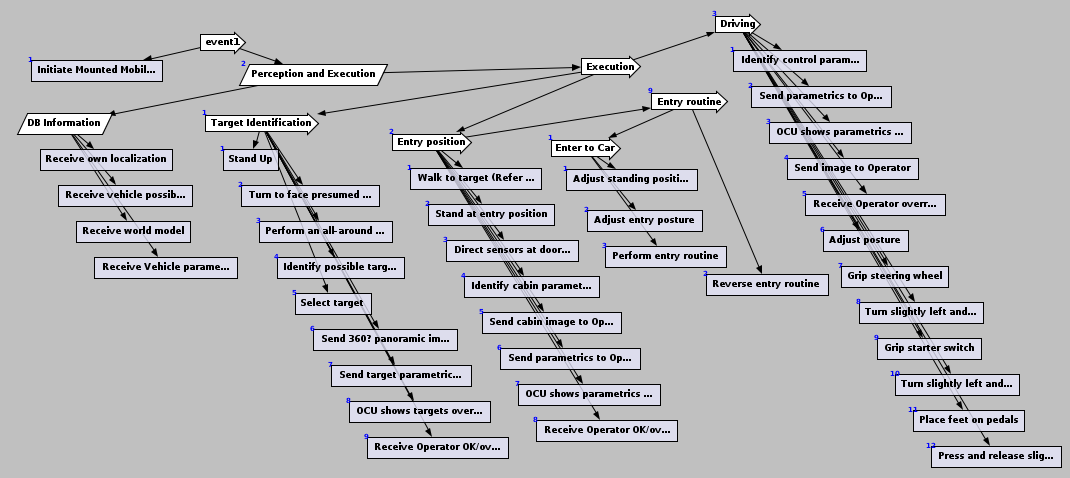
\includegraphics[width=.49\textwidth]{plan1}
	\caption{A plan for Drive challenge task, 47 nodes}
	\label{fig:drive}
\end{figure}

\begin{figure}
	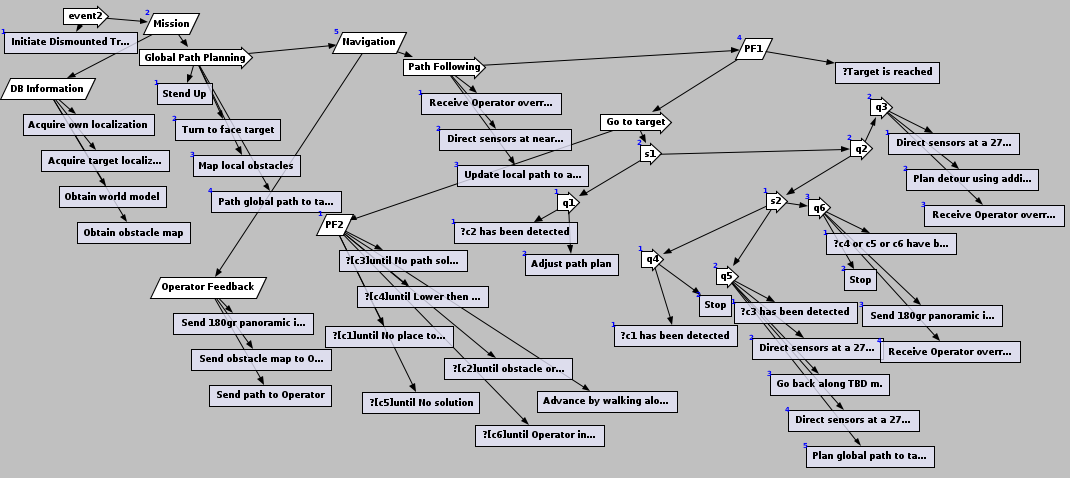
\includegraphics[width=.49\textwidth]{plan2}
	\caption{A plan for Walk challenge task, 57 nodes}
	\label{fig:walk}
\end{figure}


\begin{figure}
	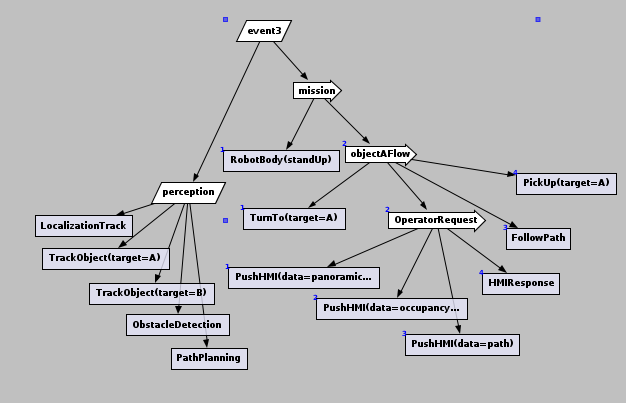
\includegraphics[width=.49\textwidth]{plan31}
	\caption{A plan for Pick-Up challenge task}
	\label{fig:pickup}
\end{figure}

In the Logistics domain, packages are to be transported by trucks or airplanes.
Hierarchical plans were generated by the JSHOP2 planner~\cite{nau2003shop2} for this domain and consisted of one parallel node (packages delivered in parallel),
with children all being sequential plans. In Figure {\ref{fig:transport}} presented a simple plan generated by JSHOP2 algorithm for accomplishing (transport-two p1 p2) from the following initial state: $\{$(package p1), (at p1 l1), (destination p1 l3), (available-truck t1), (at t1 home),
(package p2), (at p2 l2), (destination p2 l3), (available-truck t2), (at t2 home)$\}$.
The duration distribution of all primitive tasks is uniform but the support parameters were determined by the type of the task, 
in some tasks the distribution is fixed (such as for load and unload) and in others the distribution depends on the velocity of the vehicle
and on the distance to be travelled.

After running our approximation algorithm we also ran a variant
that uses an inverted version of the $\Trim$ operator, providing a {\em lower} bound of the CDF, as well as the upper bound
generated by Algorithm~\ref{alg:approx}. Running both variants allows us to bound the actual error, costing
only a doubling of the run-time. Despite the fact that our error bound is theoretically tight, in practice
and with actual distributions, according to Tables~\ref{tab:errors1} and ~\ref{tab:errors2}, the resulting error
in the algorithm was usually much better than the theoretical $\varepsilon$ bound.


We ran the exact algorithm, our approximation algorithm with $\varepsilon \in \{ 0.1, 0.01, 0.001\}$, and a simple simulation with 
$10^3$ to $10^7$ samples (number of samples is denoted by $s$ in the table), on networks from the DRC
implementation, sequence nodes with 10, 20, and 50 children (number of nodes denoted by $N$ in the table), and 20 Logistics domain plans, and
several values of $M$ (the notations $M, N$ are as in Theorem~\ref{th:TTalgcomplexity}). 
Results for the various task trees are shown in tables~\ref{tab:errors1},~\ref{tab:errors2} (error comparison) and~\ref{tab:runtimes1},~\ref{tab:runtimes2} (runtime comparison).
Errors are the maximum error in the CDF, measured from the true result when available, and from the bounds generated by the approximation algorithm using $\varepsilon = 0.0001$
when the exact algorithm timed out (over 2 hours). 
The exact algorithm times out in many cases when the number of tasks is 20 or more, except when size of the support $M$ is very small, in which case it handles some more nodes, but still cannot handle 
50 tasks even for $M=2$.
Both our approximation algorithm and the sampling algorithm handle all these cases, as our algorithm's runtime is polynomial in $N$, $M$, and ${1}/{\varepsilon}$
as is the sampling algorithm's (time linear in number of samples). 

The advantage of the approximation algorithm is mainly in providing bounds with
certainty as opposed to the bounds in-probability provided by sampling. 
Additionally, as predicted by theory, accuracy of the approximation algorithm
improves linearly with ${1}/{\varepsilon}$ (and almost linear in runtime), whereas accuracy of sampling improves only as a square root of the number of
samples. Thus, even in cases where sampling initially outperformed the approximation algorithm, increasing the required accuracy for both algorithms,
eventually the approximation algorithm overtook the sampling algorithm.


\begin{figure}[htb]
	\centering  
	
		\tikzset{
			basic/.style  = {draw, text width=5cm, font=\sffamily, rectangle},
			root/.style   = {basic, trapezium,trapezium left angle=70,trapezium right angle=-70, thin, align=center},
			level 2/.style = {basic, ,single arrow, thin, align=center,
				text width=7em},
			level 3/.style = {basic, thin, align=left,  text width=7em}
		}
		\begin{tikzpicture}
		 [
		level 1/.style={sibling distance=45mm},
		edge from parent/.style={->,draw},
		>=latex]
		
		% root of the the initial tree, level 1
		\node[root] {(transport-two p1 p2)}
		% The first level, as children of the initial tree
		child {node[level 2 ] (c1) {(transport p1)}}
		child {node[level 2] (c2) {(transport p2)}};
		
		% The second level, relatively positioned nodes
		\begin{scope}[every node/.style={level 3}]
		
		\node [single arrow, below of = c1, xshift=25pt] (c11) {(dispatch t1 l1)};
		\node [below of = c11, xshift=25pt] (c111) {(reserve t1)};
		\node [below of = c111] (c112) {(move t1 home l1
			)};
		
		\node [below of = c112, xshift=-25pt] (c12) {(load t1 p1)};
		\node [ below of = c12] (c13) {(move t1 l1 l3)};
		\node [single arrow,below of = c13] (c14) {(return t1 l1
			)};
		\node [below of = c14, xshift=25pt] (c141) {(free t1)};
		\node [below of = c141] (c142) {(move t1 l3 home
			)};
		
		
		\node [single arrow,below of = c2, xshift=25pt] (c21) {(dispatch t2 l2)};
		\node [below of = c21, xshift=25pt] (c211) {(reserve t2)};
		\node [below of = c211] (c212) {(move t2 home l2)};
		
		\node [below of = c212, xshift=-25pt] (c22) {(load t2 p2)};
		\node [below of = c22] (c23) {(move t2 l2 l3)};
		\node [single arrow,below of = c23] (c24) {(return t12 l2)};
		\node [below of = c24, xshift=25pt] (c241) {(free t2)};
		\node [below of = c241] (c242) {(move t2 l3 home)};
		
		\end{scope}
		
		% lines from each level 1 node to every one of its "children"
		\foreach \value in {1,...,4}
		\draw[->] (c1.195) |- (c1\value.west);
		\foreach \value in {1,2}
		\draw[->] (c11.195) |- (c11\value.west);
		\foreach \value in {1,2}
		\draw[->] (c14.195) |- (c14\value.west);
		
		
		\foreach \value in {1,...,4}
		\draw[->] (c2.195) |- (c2\value.west); 
		\foreach \value in {1,2}
		\draw[->] (c21.195) |- (c21\value.west);
		\foreach \value in {1,2}
		\draw[->] (c24.195) |- (c24\value.west);  
		
		\end{tikzpicture}

	\caption{A simple plan generated by JSHOP2 algorithm.
		\label{fig:transport}
	}
\end{figure}  



\begin{table*}[tbh!]
	{\footnotesize
		\begin{tabular}{|l|l|l|| p{1.5cm}|p{1.5cm}|p{1.8cm}||l|l|l|l|l|}
			\hline
			\multicolumn{1}{|c|}{\multirow{2}{*}{Task Tree}} & \multicolumn{1}{c|}{\multirow{2}{*}{$N$}} & \multicolumn{1}{c|}{\multirow{2}{*}{$M$}} & \multicolumn{3}{c|}{Approx. alg. err., given $\varepsilon$} & \multicolumn{5}{c|}{Sampling alg. err., given \# samples} \\ \cline{4-11} 
			\multicolumn{1}{|c|}{} & \multicolumn{1}{c|}{} & \multicolumn{1}{c|}{} & \multicolumn{1}{c|}{0.1} & \multicolumn{1}{c|}{0.01} & \multicolumn{1}{c|}{0.001} & \multicolumn{1}{c|}{$10^{3}$} & \multicolumn{1}{c|}{$10^{4}$} & \multicolumn{1}{c|}{$10^{5}$} & \multicolumn{1}{c|}{$10^{6}$} & \multicolumn{1}{c|}{$10^{7}$} \\ \hline \hline
			\multirow{3}{*}{Drive} & 47 & 2 & [-0.0052, 0.0086] & [-0.0004, 0.0004] & [-$3.2 {\cdot} 10^{-5}$, $3.4 {\cdot} 10^{-5}$] & 0.0206 & 0.0072 & 0.0031 & 0.0009 & 0.0001 \\ \cline{2-11} 
			& 47 & 4 & [-0.0096, 0.019] & [-0.0009, 0.0013] & [-$9.2 {\cdot} 10^{-5}$, $1.3 {\cdot} 10^{-4}$] & 0.0476 & 0.0075 & 0.0046 & 0.0011 & 0.0001 \\\cline{2-11} 
			& 47 & 10 & [-0.014, 0.028] & [-0.0014, 0.0025] & [-$9.5 {\cdot} 10^{-5}$, $1.4 {\cdot} 10^{-4}$] & 0.0236 & 0.0083 & 0.0024 & 0.0015 & 0.0003 \\ \hline
			\multirow{2}{*}{Walk} & 57 & 2 & [-0.0039, 0.004] & [-0.0003, 0.0003] & [-$3.1 {\cdot} 10^{-5}$, $3.2 {\cdot} 10^{-5}$] & 0.0166 & 0.0067 & 0.002 & 0.0008 & 0.0003 \\ \cline{2-11} 
			& 57 & 4 & [-0.0038, 0.004] & [-0.0004,  0.0004] & [-$3.6 {\cdot} 10^{-5}$, $3.9 {\cdot} 10^{-5}$] & 0.0232 & 0.0125 & 0.0022 & 0.0014 &  0.0003 \\ \cline{2-11} 
			& 57 & 10 & [-0.0047, 0.0049] & [-0.0004, 0.0005] & [-$3.8 {\cdot} 10^{-5}$, $4 {\cdot} 10^{-5}$] & 0.0255 & 0.0117 & 0.0029 & 0.0011  & 0.0003 \\ \hline
			\multirow{2}{*}{Pick Up} & 18 & 10 & {[}-0.0041, 0.0061{]} & {[}-0.0003, 0.0005{]} & {[}-$3.5 {\cdot} 10^{-5}$, $5.8 {\cdot} 10^{-5}${]} & 0.018 & 0.0054 & 0.0027 & 0.0006 & 0.0002 \\ \cline{2-11}
			& 18 & 20 & [-0.0038, 0.0031] & [-0.0006, 0.0005] & [-$3 {\cdot} 10^{-5}$, $3.5 {\cdot} 10^{-5}$] & 0.027 & 0.0046 & 0.0015  & 0.0008 & 0.0002 \\ \hline
			\multirow{2}{*}{Logistics1} & 34 & 2 & [-0.0019, 0.0019] & 0& 0& 0.0168 & 0.007 & 0.001 & 0.0009 & 0.0002 \\ \cline{2-11}  
			& 34 & 4  & [-0.0068, 0.0068]  & [-0.0006, 0.0006] & [-$3.4{\cdot} 10^{-5}$, $3.8{\cdot} 10^{-5}$] & 0.025 & 0.0057 & 0.0032 & 0.0005 & 0.0003\\ \cline{2-11}  
			& 34 & 10  & [-0.008, 0.007] & [-0.0009, 0.0007] & 0 & 0.018 & 0.011 & 0.003 &0.0009 & 0.0004\\ \hline
			\multirow{2}{*}{Logistics2} & 45 & 2 & [-0.002, 0.002] & 0& 0 & 0.013 & 0.015 & 0.004& 0.001 & 0.0003 \\ \cline{2-11}  
			& 45 & 4  & [-0.004, 0.004] & [-0.0004, 0.0004] & [-$3.3{\cdot} 10^{-5}$, $3.4{\cdot} 10^{-5}$]& 0.036 & 0.008 & 0.002 & 0.0006 &0.0002\\ \cline{2-11}  
			& 45 & 10  &[-0.005, 0.006]  & [-0.0004, 0.0006] & 0 & 0.03 & 0.013 & 0.002 &0.001 & 0.0002 \\ \hline
			%\multirow{1}{*}{Rand100-AVG} & 100 & 4 & 0.0065 & - &- &0.317 & - &- & - & - \\  \hline
			%\multirow{1}{*}{Rand200-AVG} & 200 & 4 & 0.0031 & - & -  &  0.587 & - & -& - & - \\  \hline   
		\end{tabular}
		\caption{Estimation errors}
		\label{tab:errors1}
	}
	%\vspace*{-0.5cm} 
\end{table*}





\begin{table*}[htb!]
	{\footnotesize
		\begin{tabular}{|l|l|l|l||l|l|l||l|l|l|l|l|}
			\hline
			\multicolumn{1}{|c|}{\multirow{2}{*}{Task Tree}} & \multicolumn{1}{c|}{\multirow{2}{*}{$N$}} & \multicolumn{1}{c|}{\multirow{2}{*}{$M$}} & \multirow{2}{*}{Exact} & \multicolumn{3}{c|}{Approx. alg., with $\varepsilon$} & \multicolumn{5}{c|}{Sampling alg., with \# samples} \\ \cline{5-12} 
			\multicolumn{1}{|c|}{} & \multicolumn{1}{c|}{} & \multicolumn{1}{c|}{} &  & \multicolumn{1}{c|}{0.1} & \multicolumn{1}{c|}{0.01} & \multicolumn{1}{c|}{0.001} & \multicolumn{1}{c|}{$10^{3}$} & \multicolumn{1}{c|}{$10^{4}$} & \multicolumn{1}{c|}{$10^{5}$} & \multicolumn{1}{c|}{$10^{6}$} & \multicolumn{1}{c|}{$10^{7}$} \\ \hline \hline
			\multirow{2}{*}{Drive} & 47 & 2 & 1.49 & 0.141 & 1.14 & 1.49 & 0.187 & 1.92 & 19.11 & 190.4 & 1905 \\ \cline{2-12} 
			& 47 & 4 & 18.9 & 0.34 & 7.91 & 16.11 & 0.21 & 2.1 & 20.95 &  211.5 & 2113.6\\ \cline{2-12}
			& 47 & 10 & $> 2$h & 1.036 & 32.94 & 390.5 & 0.28 & 2.81 & 28.6 &279.1  &  2844.4  \\ \hline
			\multirow{2}{*}{Walk}  & 57 & 2& 4.46 & 0.33 & 3.1 & 4.03 & 0.205 & 2.06 & 20.86 & 208.1 & 2082.7  \\ \cline{2-12} 
			& 57 & 4  & 183.5 & 0.983 & 18.42 & 95.11 & 0.23 & 2.34 & 23.03 & 230.4 & 2352.4 \\ \cline{2-12} 
			& 57 & 10 & $> 2$h & 8.13 & 128.99 & 3668.2 & 0.293 & 2.92 & 29.16 & 291.3 & 2902.7 \\ \hline
			\multirow{2}{*}{Pick Up} & 18 & 10 & 5.76 & 0.022 & 0.193 & 1.133 & 0.103 & 0.983 & 9.8 & 101.9 & 1006.8 \\ \cline{2-12} 
			& 18 & 20 & 27.88 & 0.046 & 0.4 & 3.15 & 0.132 & 1.33 & 13.25 & 130.4 & 1305.9 \\ \hline
			\multirow{2}{*}{Logistics1} & 34 & 2 & 0.014 & 0.007 &  0.009 & 0.009 & 0.239 & 2.03 & 19.3 & 193.9 & 1767 \\ \cline{2-12} 
			& 34 & 4 & 22.98 & 0.048 & 1.3 & 13.1 & 0.2 &  2 & 20 & 205 &1928\\ \cline{2-12}  
			& 34 & 10 & $> 4$h & 0.25 & 8.26 & 475 & 0.26 & 2.64 & 26.4 & 267 & 2649 \\ \hline 
			\multirow{2}{*}{Logistics2} & 45 & 2 & 0.07 &  0.02 &  0.06 & 0.06 & 0.23 & 2.35 & 23.4 & 234.7 & 2196 \\ \cline{2-12} 
			& 45 & 4 & 373.3& 0.2 & 7 & 82.9 & 0.25 & 2.5 & 25.6 & 256 & 2393\\ \cline{2-12}  
			& 45 & 10 & $> 4$h & 2.19 & 120 & 6101 & 0.31 & 3.12 & 31.3 &314 & 3139\\ \hline
		\end{tabular}
		\caption{Runtime comparison (run times in seconds)}
		\label{tab:runtimes1}
	}
	
\end{table*}

\begin{table*}[tbh!]
	{\footnotesize
		\begin{tabular}{|l|l|l|| p{1.5cm}|p{1.5cm}|p{2.4cm}||l|l|l|}
			\hline
			\multicolumn{1}{|c|}{\multirow{2}{*}{Task Tree}} & \multicolumn{1}{c|}{\multirow{2}{*}{$N$}} & \multicolumn{1}{c|}{\multirow{2}{*}{$M$}} & \multicolumn{3}{c|}{Approx. alg. err., given $\varepsilon$} & \multicolumn{3}{c|}{Sampling alg. err., given \# samples} \\ \cline{4-9} 
			\multicolumn{1}{|c|}{} & \multicolumn{1}{c|}{} & \multicolumn{1}{c|}{} & \multicolumn{1}{c|}{0.1} & \multicolumn{1}{c|}{0.01} & \multicolumn{1}{c|}{0.001} & \multicolumn{1}{c|}{$10^{3}$} & \multicolumn{1}{c|}{$10^{4}$} & \multicolumn{1}{c|}{$10^{5}$} \\ \hline \hline
			\multirow{2}{*}{Seq 10} & 10 & 4 & [-0.027, 0.041] & [-0.0027, 0.0041] & [-$2.2 {\cdot} 10^{-4}$, $2.5 {\cdot} 10^{-4}$] & 0.0224 & 0.008 & 0.0017  \\ \cline{2-9} 
			& 10 & 10 &[-0.0316, 0.0615]  & [0.0033, 0.0067] & [$-2.6 {\cdot} 10^{-4}$, $5.2 {\cdot} 10^{-4}$] & 0.027 & 0.0117 & 0.0038  \\ \hline 
			\multirow{2}{*}{Seq 20} & 20 & 2 & [-0.02, 0.0373 ] & [-0.0015, 0.0026] & [-$1.6 {\cdot} 10^{-4}$, $2.6 {\cdot} 10^{-4}$]  & 0.0266 & 0.0077 &  0.003   \\ \cline{2-9} 
			& 20 & 4 & [-0.026, 0.025] & [-0.0025, 0.0025]  & [-$2.7{\cdot} 10^{-4}$, $2.3 {\cdot} 10^{-4}$] & 0.039 & 0.01 & 0.002 \\ \cline{2-9} 
			& 20 & 10   & [-0.027, 0.027] & [-0.0028, 0.0027] & [-$3 {\cdot} 10^{-4}$, $2.5 {\cdot} 10^{-4}$] & 0.032 & 0.007 & 0.0042  \\ \hline
			\multirow{2}{*}{Seq 50} & 50 & 2 & [-0.032, 0.032] & [-0.0028, 0.0028] & [-$2.8 {\cdot} 10^{-4}$, $2.4 {\cdot} 10^{-4}$]  & 0.0193 & 0.007 & 0.0024  \\ \cline{2-9}  
			& 50 & 4  & [-0.035, 0.035]  & [-0.0036, 0.0035] &[-$3.9 {\cdot} 10^{-4}$, $3.2 {\cdot} 10^{-4}$]  & 0.0236 & 0.0064 & 0.0023 \\ \cline{2-9}  
			& 50 & 10  & [-0.037, 0.037] & [-0.004, 0.0039] & [-$4.2 {\cdot} 10^{-4}$, $3.5 {\cdot} 10^{-4}$] & 0.017 & 0.007  & 0.005  \\ \hline
			\multirow{1}{*}{Rand50-AVG} & 50 & 4 & 0.007 & 0.0007 &  0 & 0.0243 & 0.0084 & 0.0024 \\   \hline
			
		\end{tabular}
		\caption{Estimation errors for sequential plans}
		\label{tab:errors2}
	}
	%\vspace*{-0.5cm} 
\end{table*}




\begin{table*}[htb!]
	{\footnotesize
		\begin{tabular}{|l|l|l|l||l|l|l||l|l|l|}
			\hline
			\multicolumn{1}{|c|}{\multirow{2}{*}{Task Tree}} & \multicolumn{1}{c|}{\multirow{2}{*}{$N$}} & \multicolumn{1}{c|}{\multirow{2}{*}{$M$}} & \multirow{2}{*}{Exact} & \multicolumn{3}{c|}{Approx. alg., with $\varepsilon$} & \multicolumn{3}{c|}{Sampling alg., with \# samples} \\ \cline{5-10} 
			\multicolumn{1}{|c|}{} & \multicolumn{1}{c|}{} & \multicolumn{1}{c|}{} &  & \multicolumn{1}{c|}{0.1} & \multicolumn{1}{c|}{0.01} & \multicolumn{1}{c|}{0.001} & \multicolumn{1}{c|}{$10^{3}$} & \multicolumn{1}{c|}{$10^{4}$} & \multicolumn{1}{c|}{$10^{5}$}  \\ \hline \hline
			\multirow{2}{*}{Seq 10} & 10 & 4 & 0.23 & 0.003 & 0.02 & 0.148  & 0.054 & 0.545 &5.336  \\ \cline{2-10} 
			& 10 & 10 & 10.22 & 0.008 & 0.073 & 0.692 & 0.071 & 0.724 & 7.18  \\ \hline
			\multirow{2}{*}{Seq 20} & 20 & 2 & 0.23 & 0.003 & 0.02 & 0.285  & 0.054 & 0.545 & 9.62  \\ \cline{2-10} 
			& 20 & 4 & $> 2$h & 0.011 & 0.106 & 1.208 & 0.105 & 1.066 & 10.74 \\ \cline{2-10} 
			& 20 & 10 & $> 2$h & 0.035 & 0.331 & 4.67 & 0.145 & 1.473 & 14.38  \\ \hline
			\multirow{2}{*}{Seq 50} & 50 & 2 & $> 2$h & 0.028 &  0.28 & 3.593  & 0.236 & 2.366 & 24.71  \\ \cline{2-10} 
			& 50 & 4 & $> 2$h & 0.079 & 0.81 & 11.145 & 0.265 & 2.68 & 26.84\\ \cline{2-10}  
			& 50 & 10 & $> 2$h & 0.227 & 3.1 & 38.01 & 0.354 & 3.63 & 35.63  \\ \hline
			\multirow{1}{*}{Rand50-AVG} & 50 & 4 & $>2$h & 1.1544 & 19.77 & 390.58 & 5.676 & 55.021 & 590.17 \\   \hline
		\end{tabular}
		\caption{Runtime comparison (run times in seconds) for sequential plans}
		\label{tab:runtimes2}
	}
\end{table*}

%The following graphs present more vividly the results for the task trees used as execution plans in the DARPA robotics challenge. The horizontal axis represents the run-time of the algorithm (exact, sampling, approximation) and the vertical axis represent the upper bound error. Clearly, in all graphs our approximation algorithm for $\varepsilon=0.01$ and $\varepsilon=0.001$ provides very small error comparing to the exact result and the run-time is lower. In addition, in most graphs (7/8), the sampling results are less accurate and the run-time is higher comparing to our approximation algorithm results. The only exception is in the Drive task tree with M=10 and $\varepsilon=0.1$. Our result is less accurate and the run-time is higher than the sampling algorithm for $10^3$ samples. However, for $10^4$ the run-time of our approximation algorithm is lower than the sampling algorithm and for $\varepsilon=0.01$ and $\varepsilon=0.001$ our results are better than the sampling results.



\section{Dependencies and other generalizations}\label{sec:generalizations}

Computing the distribution of the makespan in trees is considered a trivial problem in some contexts
in probabilistic reasoning~\cite{Pearl}.
Specifically, given the task network, such as the one in Figure~\ref{fig:task-network},
it is straightforward to represent the 
distribution using a Bayes network (BN) that has one node
per task where the {\em children} of a node $v$ in the 
task network are represented by BN nodes that are {\em parents} of
the BN node representing $v$. This results in a tree-shaped BN, 
where it is well known that probabilistic reasoning can be done in time linear
in the number of nodes, e.g., by belief propagation (message passing)~\cite{Pearl,Kim}. 
However, there is a difficulty, ignored in this literature, in the potentially exponential size
of variable domains, which our algorithm, essentially a limited form
of approximate belief propagation from primitive task variables to the root, avoids by trimming.

\begin{figure}
\centering
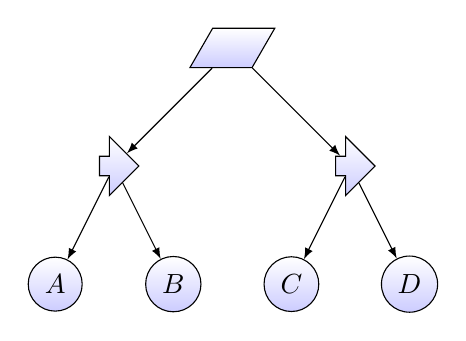
\begin{tikzpicture}[
    level/.style={sibling distance=30mm/#1},
    edge from parent/.style = {draw, -latex},
    sloped,
    every node/.style = {trapezium, trapezium left angle=60, trapezium right angle=-60, draw, align=center, top color=white, bottom color=blue!20,minimum height=0.5cm}
]
   \node {}  
   child { node [single arrow] {} 
        child{ node [circle] {$A$}}
        child{ node [circle] {$B$}}
    }    
    child  { node [single arrow] {} 
        child{ node [circle] {$C$}}
        child{ node [circle] {$D$}}
    }
    ;
\end{tikzpicture}
\caption{A simple task network.}
\label{fig:task-network}
\end{figure}

Looking at makespan distribution computation as probabilistic reasoning leads immediately to 
the question on how to handle task completion times that have dependencies, represented as a BN. 
Since reasoning in BNs is NP-hard even for binary-valued variables~\cite{Dagum.aij,Cooper.ai}, 
this is hard in general.
But for cases where the BN toplogy is tractable, such as for BNs with a small cutset %~\cite{??}
BNs with bounded treewidth~\cite{Bodlaender:2006:TCA:2092758.2092759},
or directed-path singly connected BNs~\cite{ShimonyDomshlak.aiRN2003},
a deterministic polynomial-time approximation scheme for 
the makespan distribution may be achievable.

\begin{figure}
\centering
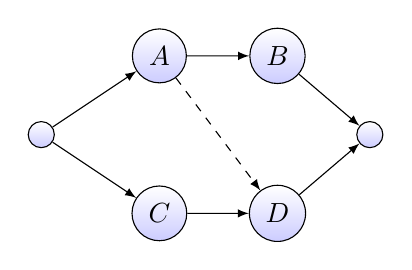
\begin{tikzpicture}[
    level/.style={sibling distance=20mm/#1},
    edge from parent/.style = {draw, -latex},
    sloped,
    grow=right,
    every node/.style = {circle, draw, align=center, top color=white, bottom color=blue!20}
]
   \node (S) {}  
        child{ node (C)  {$C$}
        	child{ node (D)  {$D$}  }
        }
        child{ node (A)  {$A$}
        	child{ node (B)  {$B$} }
        }

    ;
    
    \node (T) [right=4cm] {};
    
    \path [draw, -latex] (D) -- (T);
    \path [draw, -latex] (B) -- (T);
    \path [draw, -latex, dashed] (A) -- (D);
\end{tikzpicture}
\caption{A petri-net graph.}
\label{fig:petri-net-graph}
\end{figure}

\begin{figure}
\centering
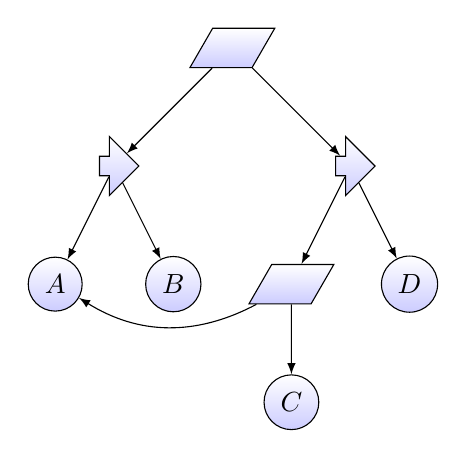
\begin{tikzpicture}[
    %sibling distance        = 6em,
    %level distance          = 4em,
    level/.style={sibling distance=30mm/#1},
    edge from parent/.style = {draw, -latex},
    sloped,
    every node/.style = {trapezium, trapezium left angle=60, trapezium right angle=-60, draw, align=center, top color=white, bottom color=blue!20,minimum height=0.5cm}
]
   \node {}  
   child { node [single arrow] {} 
        child{ node (A) [circle] {$A$}}
        child{ node [circle] {$B$}}
    }    
    child  { node [single arrow] {} 
        child{  node (X2) {}         
        	child {node [circle] {$C$}}
        }
        child{ node [circle] {$D$}}
    }
    ;
    
    \path [draw, -latex] (X2) [bend left] edge (A);
\end{tikzpicture}
\caption{A non-hierarchical task network}
\label{fig:non-tree-TN}
\end{figure}


\begin{figure}
\centering
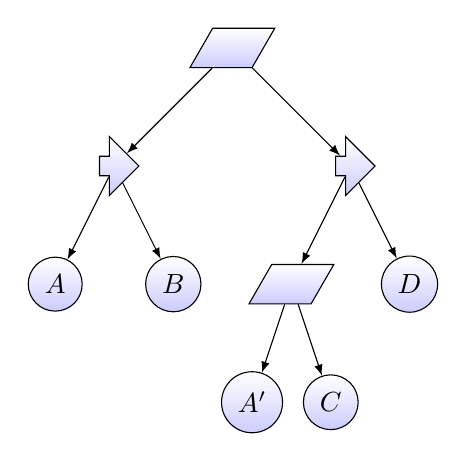
\begin{tikzpicture}[
    level/.style={sibling distance=30mm/#1},
    edge from parent/.style = {draw, -latex},
    sloped,
    every node/.style = {trapezium, trapezium left angle=60, trapezium right angle=-60, draw, align=center, top color=white, bottom color=blue!20,minimum height=0.5cm}
]
   \node {}  
   child { node [single arrow] {} 
        child{ node (A) [circle] {$A$}}
        child{ node [circle] {$B$}}
    }    
    child  { node [single arrow] {} 
        child{  node (X2) {}         
             child {node [circle] {$A'$}}
        	child {node [circle] {$C$}}
        }
        child{ node [circle] {$D$}}
    }
    ;
    
    
\end{tikzpicture}
\caption{Representing ``shared'' tasks  using correlated random variables}
\label{fig:task-network-with-copy}
\end{figure}



Here we motivate and handle a special case of a small cutset. 
Specifically, suppose that, in addition to the tree, we allow a small number of dependencies
between primitive task distributions. Does our algorithm generalize to this case?
The importance of this question is because such an extension is natural in some contexts. For example,
in the logistics case we have a 2-level tree, with a toplogy similar to that of Figure ~\ref{fig:task-network}.
The children of the sequence nodes are primitive tasks such as
``drive delivery truck 1 from Boston to NY'' (suppose this is primitive task A in  Figure ~\ref{fig:task-network}).
Now, the duration of this action is a random variable
that depends on the state of traffic at the time the action is taken. Suppose that another
primitive action (e.g. primitive task C) is ``drive delivery truck 2 from Boston to NY'' which is to occur roughly at the
same time as the first action. Since traffic conditions are likely to be very similar, the
duration of the actions may be correlated, and we need to be able to take
this dependency into account.

Another case where we have dependency is when the same primitive action is 
used in more than one composite task. Although this state cannot be represented in
strict hierarchies, recall that timing relationships represented by HTNs can also be
represented by directed acyclic perti nets. For example, the task network of Figure~\ref{fig:task-network}
can be represented by the perti net of Figure~\ref{fig:petri-net-graph} (without the shaded arc). However, perti nets allow more general
timing constraints: the language of trees is equlivalent to perti nets with a series-parallel
graph structure. Adding the shaded arc from A to D in the petri net of Figure~\ref{fig:petri-net-graph}, 
we get a graph that is not series-parallel. Its equivalent in HTNs would be the non-tree structure
shown in Figure~\ref{fig:non-tree-TN}, that shares primitive task A between composite tasks. 
The latter could be converted into a pure tree-shape by adding a task A' that mirrors task A,
i.e. has a duration exactly equal to that of A (Figure~\ref{fig:task-network-with-copy}).

This case, as well as generalizations thereof where the number of correlated variables is small,
we can handle by a scheme known as {\em conditioning}, adapted to our approximation scheme.
For example, in cutset conditioning, a separate reasoning problem is generated
for every possible value instantiation over all the cutset variables. The results
are combined by weighted averaging. We propose to do the same in our case, but must prove
that the approximation quality is maintained, as we indeed do below.

We thus assume that all primitive task durations are independent, when conditioned on
a small cutset $Y$ of the primitive task durations. The joint duration distribution over $Y$
can be provided by a BN, or a complete table, or any other representation. We assume
that the cardinality of the set $Y$ is sufficiently small that the joint domain
size $m^{|Y|}$ is managable, in terms of memory and computation time if we have to
iterate over all domain values. We are also given the duration distribution for any
other task, given every possible value assignment $y$ to the variables in $Y$.
Together, this information fully defines the joint probability of all the 
primitive task durations. 

For example, in the case of Figure~\ref{fig:task-network-with-copy}, we can set $Y=\{ A\}$, so $Y$ is a singleton set.
This is a somewhat degenerate example case, as
the joint distribution can be represented trivially using $P(A'=a'|A=a)=1$,
as  all other primitive task duration variables are independent of $A$.

Let $X$ be the random variable denoting the makespan distribution of the
root of the task network. We wish to estimate $F_X$, the cumulative distribution of $X$.
Our approximation algorithms for trees without dependency can estimate an
upper and lower bounds approximations. With dependencies, we cannot do so directly.
However, consider an assignment $Y=y$, for some value $y\in D(Y)$. We are given the conditional
distribution $Z|Y=y$ for all the rest of the primitive tasks, which are now
independent given $Y=y$. Consider the distribution:
\[
F_{X|Y=y}(x) = P(X\leq x| Y=y)
\]
For each value $Y=y$ we can run the approximation algorithm, to get upper and lower bounds.
$F^-_{X|Y=y}(x)$ and  $F^+_{X|Y=y}(x)$. Due to Theorem~\ref{th:TNapprox}, we have
the following property, for all $x$:
\[
F^-_{X|Y=y}(x) \approx _\varepsilon F_{X|Y=y}(x) \approx _\varepsilon F^+_{X|Y=y}(x)
\]
Now let:
\[
F^-_{X}(x) \sum_{y\in D(Y)} P(Y=y) F^-_{X|Y=y}(x)
\]
and likewise:
\[
F^+_{X}(x) \sum_{y\in D(Y)} P(Y=y) F^+_{X|Y=y}(x)
\]

\hl{To Eyal:} the $\approx$ symbol is not defined.

\begin{theorem}
Computing these values takes time $O(m^{|Y|})t$, where $t$ is the runtime
of our tree task network algorithm. The resulting approximation obeys, for all $x$:
\[
F^-_{X}(x) \approx _\varepsilon F_{X}(x) \approx _\varepsilon F^+_{X}(x)
\]
\end{theorem}

Proof: the runtime bound is obvious, as a trivial implementation simply encurs $m^{|Y|}$
runs of the tree task network algorithm. The approximation bounds follow
from the bounds for individual values $Y=y$, and from a convexity argument.
For example, by construction, we have:
\[
F^-_{X}(x) -  F_{X}(x) =  \sum_{y\in D(Y)} P_{Y}(y)(F^-_{X|Y=y}(x) - F_{X|Y=y}(x))
\]
The right hand side is a convex sum of quantities that are all between 0 and $\varepsilon$, which therefore
must also be between 0 and $\varepsilon$.

\section{Discussion and Related Work}\label{sec:discussion}

Numerous issues remain unresolved, briefly discussed below.
Trivial improvements to the $\Trim$ operator are possible, such as the inverse version of the operator used to
generate a lower bound for the empirical results. Other candidate improvements are not performing trimming
(or even stopping a trimming operation) if the current support size is below $1/\varepsilon$, which may increase accuracy but also
the runtime. Another point is that in the combined algorithm, space and time complexity can be reduced by adding some $\Trim$ operations,
especially after processing a parallel node, which is not done in our version. This may reduce accuracy, 
a trade-off yet to be examined.
Another option is, when given a specific threshold, trying for higher accuracy in just the region of the
threshold, but how to do that is non-trivial. For {\em sampling} schemes such methods are known, including adaptive 
sampling~\cite{bucher1988adaptive,lipton1990practical},
stratified sampling, and other schemes.
It may be possible to apply such schemes to deterministic algorithms as well - an interesting issue for future work.

Extension to continuous distributions: our algorithm can handle them by
pre-running a version of the $\Trim$ operator on the primitive task distribution. Since one cannot iterate over support values
in a continuous distribution, start with the smallest support value (even if it is $- \infty$), and find the value at which the CDF
increases by $\varepsilon$. This requires access to the inverse of the CDF, which is available, either exactly or approximately,
for many types of distributions. %In fact, this is precisely how Gaussian distributions were handled in our
%empirical evaluation.

We showed that the expectation problem is also NP-hard.
A natural question is on approximation algorithms for the expectation problem, but the answer here is not so obvious.
Sampling algorithms may run into trouble if the target distribution contains major outliers, i.e. values very far from
other values but with extremely low probability. Our approximation algorithm can also be used as-is to estimate
the CDF and then to approximate the expectation, but we do not expect it to perform well because our current $\Trim$
operator only limits the amount of probability mass moved at each location to $\varepsilon$, but does not limit the
``distance'' over which it is moved. The latter may be arbitrarily bad for estimating the expectation.
Possibly adding simple binning schemes to the $\Trim$ operator in addition to limiting the moved probability mass to $\varepsilon$
may work, another issue for future research. 

Related work on computing makespan distributions includes~\cite{hong2013computing}, which examines sum of  Bernoulli distributed r.v.s.
Other work examines both deterministic~\cite{mercier2007discrete} and  Monte-Carlo techniques~\cite{bucher1988adaptive,lipton1990practical}. 
Distribution of maximum of r.v.s was studied in~\cite{devroye1980generating}, with a focus mostly on continuous distributions.

Complexity of finding the probability that the makespan is under a given threshold in task networks was shown to
be NP-hard in~\cite{hagstrom1988computational}, even when the completion time of each task has a Bernoulli distribution.
Nevertheless, our results are orthogonal as the source of the complexity in~\cite{hagstrom1988computational} is in the graph structure,
whereas in our setting the complexity is due to the size of the support. In fact for linear plans (an NP-hard case in our setting),
the probability of meeting the deadline can be computed in low-order polynomial time for Bernoulli distributions, using straightforward dynamic programming.
Makespan distributions in series parallel networks in the i.i.d. case was examined in~\cite{gutjahr1992average}, without   
considering algorithmic issues. There is also a significant body of work on estimating the makespan of plans and schedules
\cite{herroelen2005project,fu2010towards,beck2007proactive}, within a context of a planner or scheduler. The analysis in these papers is
based on averaging or on limit theorems, and does not provide a guaranteed approximation scheme. 
Temporal planing and in particular TPNs (temporal plan network) are presented in
\cite{kim2001executing}, the model is similar to ours, but the focus is on lower/upper bounds, rather than probability distributions. 
Hierarchical constraint-based plans in \hl{MAPGEN}~\cite{bresina2005mixed} allow for more
general dependencies than series-parallel, providing additional expressive power but making the deadline problem even harder.

The research literature contains numerous {\em randomized} approximation schemes that handle dependencies~\cite{Pearl,Yuan20061189}, especially for
the case with {\em no evidence}. In fact, our implementation of the sampling scheme in ROBIL handled dependent durations.
It is unclear whether such sampling schemes can be adapted to handle dependencies {\em and} arbitrary evidence, such as: ``the completion time of
compound task $X$ in the network is known to be exactly one hour from now''.


Finally, one might consider additional commonly used utility functions, such as a ``soft'' deadline: the utility is a constant $U$ before the deadline $T$, decreasing linearly to 0
until $T+G$ for some ``grace'' duration $G$, and 0 thereafter.
\paragraph{Acknowledgments.} This research was supported by the ROBIL project, and by the Lynne and William Frankel Center for Computer Science at Ben-Gurion University.
%\clearpage
\small
\bibliographystyle{named}
\bibliography{ijcai15}

\end{document}

